%  LaTeX support: latex@mdpi.com 
%  For support, please attach all files needed for compiling as well as the log file, and specify your operating system, LaTeX version, and LaTeX editor.

%=================================================================
\documentclass[applsci,article,submit,pdftex,moreauthors]{Definitions/mdpi} 
% For posting an early version of this manuscript as a preprint, you may use "preprints" as the journal and change "submit" to "accept". The document class line would be, e.g., \documentclass[preprints,article,accept,moreauthors,pdftex]{mdpi}. This is especially recommended for submission to arXiv, where line numbers should be removed before posting. For preprints.org, the editorial staff will make this change immediately prior to posting.


%=================================================================
% MDPI internal commands
\firstpage{1} 
\makeatletter 
\setcounter{page}{\@firstpage} 
\makeatother
\pubvolume{1}
\issuenum{1}
\articlenumber{0}
\pubyear{2022}
\copyrightyear{2022}
%\externaleditor{Academic Editor: Firstname Lastname}
\datereceived{} 
\dateaccepted{} 
\datepublished{} 
%\datecorrected{} % Corrected papers include a "Corrected: XXX" date in the original paper.
%\dateretracted{} % Corrected papers include a "Retracted: XXX" date in the original paper.
\hreflink{https://doi.org/} % If needed use \linebreak
%\doinum{}
%------------------------------------------------------------------
% The following line should be uncommented if the LaTeX file is uploaded to arXiv.org
%\pdfoutput=1

%=================================================================
% Full title of the paper (Capitalized)
\Title{Controlling remotely operated vehicles with deterministic artificial intelligence}

% MDPI internal command: Title for citation in the left column
\TitleCitation{Controlling remotely operated vehicles with deterministic artificial intelligence}

% Author Orchid ID: enter ID or remove command
\newcommand{\orcidauthorA}{0000-0002-8043-1411} % Add \orcidA{} behind the author's name
\newcommand{\orcidauthorB}{0000-0002-4681-7919} % Add \orcidB{} behind the author's name

% Authors, for the paper (add full first names)
\Author{Shay Osler $^{1}$\orcidA{}, Timothy Sands $^{2,}$*$^{,}$\orcidB{}}

%\longauthorlist{yes}

% MDPI internal command: Authors, for metadata in PDF
\AuthorNames{Shay Osler, Timothy Sands}

% MDPI internal command: Authors, for citation in the left column
\AuthorCitation{Osler, S.; Sands, T.}
% If this is a Chicago style journal: Lastname, Firstname, Firstname Lastname, and Firstname Lastname.

% Affiliations / Addresses (Add [1] after \address if there is only one affiliation.)
\address{%
$^{1}$ \quad School of Electrical and Computer Engineering, Cornell University; Ithaca NY, 14853; sno5@cornell.edu\\
$^{2}$ \quad Department of Mechanical and Aerospace Engineering, Naval Postgraduate School, Monterey, USA}

% Contact information of the corresponding author
\corres{Correspondence: tasands@nps.edu}

% Abstract (Do not insert blank lines, i.e. \\) 
\abstract{Unmanned ocean vehicles can be guided and controlled autonomously or remotely, and even remote operation can be automated significantly. Classical methods use trajectory tracking errors in negative feedback. Recently published methods are proposed instead. Deterministic (non-stochastic) artificial intelligence (DAI) combines optimal learning with an asserted self awareness statement in the form of the governing mathematical model (based on physics in this instantiation) to allow control that can be alternatively adaptive (i.e. capable of reacting to changing system dynamics) or learning (i.e. able to provide information about what aspects of the system dynamics have changed). In this manuscript deterministic artificial intelligence is applied to the heading control of a simulated remotely operated underwater vehicle (ROV). Research is presented illustrating autonomous control of a Seabotix vLBV 300 remotely operated vehicle within milli-degrees on the very first step of a shaped square wave command and error decreased an additional sixty-two percent by the third step of the square wave command.}

% Keywords
\keyword{Marine engineering; artificial intelligence; dynamics; guidance and control; ocean vehicles }

%%%%%%%%%%%%%%%%%%%%%%%%%%%%%%%%%%%%%%%%%%
% Only for the journal Applied Sciences:
\featuredapplication{Autonomous unmanned vehicles, deterministic artificial intelligence}
%%%%%%%%%%%%%%%%%%%%%%%%%%%%%%%%%%%%%%%%%%

\begin{document}
%%%%%%%%%%%%%%%%%%%%%%%%%%%%%%%%%%%%%%%%%%

\begin{figure}[h]
  \widefigure
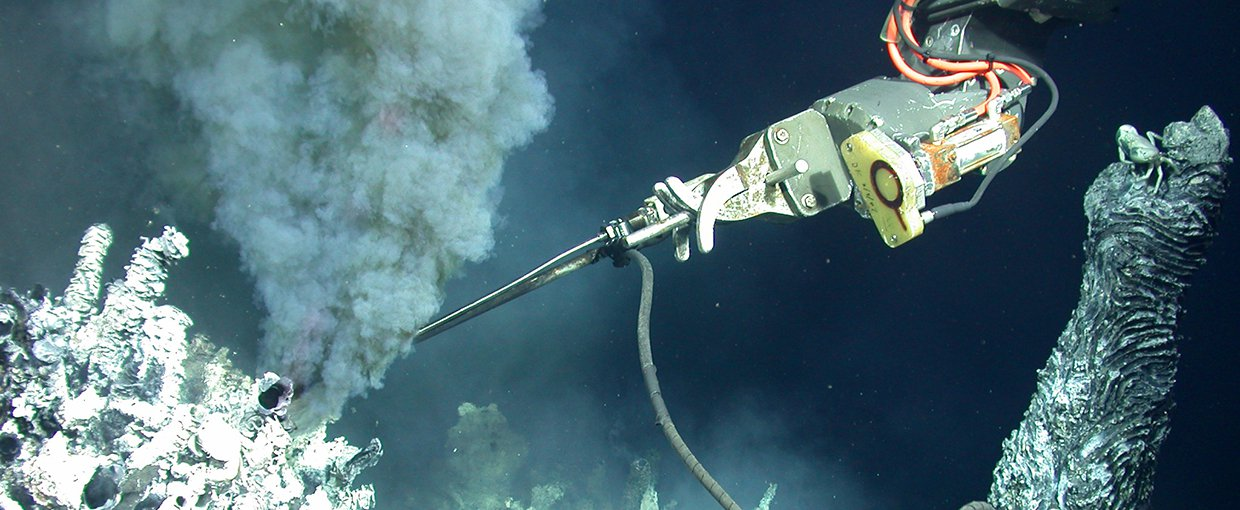
\includegraphics[width=10cm]{NASA Smoker subsampling-2.jpg}
\caption{NASA remotely operated vehicle sampling deep sea black smokers.\cite{Gronstal22} Image used for educational purposes in accordance with NASA Media Usage Guidelines \cite{NASA22}}
\label{fig:NASA Smoker subsampling-2}
\end{figure}

\section{Introduction}
Unmanned vehicles are increasingly popular in society and have proven especially useful in dangerous environments. Exploring for life deep at the bubbling chimneys of magma-heated water in the very deep, dark depths of the ocean \cite{Gronstal22} acts as prototype practice for deep space exploration by such unmanned systems as depicted in figure \ref{fig:NASA Smoker subsampling-2}. Planning to explore distant planets and moons like Europa and Enceladus, the National Aeronautics and Space Administration (NASA) uses the BRUIE underwater rover to practice looking for life under the ice in Antarctica. The BRUIE rover is depicted in figure \ref{fig:NASAbruie20191118} in an Arctic lake near Barrow, Alaska in 2015.\cite{NASA19} Such dangerous environments illustrate the importance of highly capable, advanced systems automating as much activity as possible. The popularity of using such vehicles is due in part to their very long history of technological understanding and development, being governed by fundamental principles developed hundreds of years ago. Vehicle translation is governed by principles developed by Newton in 1687 \cite{Newton87}, while rotation is governed by principles elaborated by Euler in 1776 \cite{Euler76}. The two natures of motion (translation and rotation) was expressed very early by Chasles in 1830 \cite{Chasles30} as coupled and nonlinear and shortly afterwards embodied by Coriolis in a now famous theorem. \cite{Coriolis35} Hamilton introduced alternative formulation methods in 1834 using energy \cite{Hamilton34}, while Lagrange introduced a presentation using energy that more closely resembled Newton's original formulation \cite{Lagrange11} - \cite{Lagrange15}, and in the last century Kane \cite{Kane59} - \cite{Kane85} provided the latest parameterization of the same natural relationships very often referred to as a Lagrangian formulation \cite{Lagrange11} - \cite{Lagrange15} of D'Alembert's principle, which was introduced in 1743 and published in 1747 \cite{D'Alembert47a} - \cite{D'Alembert47b} and 1750. \cite{D'Alembert50} These fundamental and now well-understood principles of mechanics embodied the approaches to control themselves in an open-loop, feedforward sense, as expressed in the 1950's and 1960's respectively by Bellman in the West \cite{Bellman57} and Pontryagin in the East \cite{Pontryagin62}. Pontryagin's work particularly applied to highly flexible robotic vehicles \cite{Sands19} sprung from their foundation of the core principles of adaptive techniques late in the last century \cite{Slotine90} - \cite{Fossen93} 

A recent lineage of adaptive controls applied to robotic systems \cite{Slotine90, Slotine91} and spacecraft \cite{Fossen93, Sands09} illustrated an ability to autonomously recover from significant damage without assistance. \cite{Nakatani14}. The foundation of those methods was unique manifestations of the governing differential equations of motion in a feedforward fashion as controls, augmented with classical feedback rules used to adapt the feedforward controls. Highlighting and amplifying this foundation, \cite{Cooper17} demonstrated feedforward controls comprised of the governing differential equations of motion driven by autonomously generated trajectory commands was superior to linear-quadratic optimal feedback control. Later \cite{Smeresky20} developed optimal (in a 2-norm sense) feedback to realize adaption, replacing the former adaptive methods based in classical feedback. In 2020, the combined method, newly labeled deterministic artificial intelligence \cite{Sands20}, comprised of self-awareness statements (the feedforward codification of the governing differential equations) plus optimal learning (through feedback), was applied to unmanned ocean vehicles \cite{Sands20} as an embodied update to classical \cite{Sands18} and optimal (so-called "modern") approaches \cite{Fossen94}. 

Deterministic artificial intelligence \cite{Sands20} is thus an alternative to adaptive control \cite{Slotine90} - \cite{Nakatani14} and classical control schemes \cite{Sands18} and is based on the observation that if one can discern the governing mathematical equations for a system (using any of the cited approaches \cite{Newton87} - \cite{Pontryagin62}) then one could use those governing equations themselves as a control law (in both feedforward \cite{Cooper17} and feedback senses \cite{Smeresky20}), which is particularly effective if the governing mathematical relationship is stipulated by physics. This allows the design of a feedforward controller that might perfectly track a desired trajectory \cite{Sands21}-\cite{Shah21} simply by plugging prescribed desired velocity and acceleration into the system’s governing equations, and then using them, calculating the required control forces and torques. Deterministic artificial intelligence first asserts the general structure of the system dynamics, then uses some form of learning to determine the parameters of the model. \cite{Smeresky20} Assuming the chosen model structure is sufficiently comprehensive to capture the dominant system dynamics, a deterministic artificial intelligence controller will be able to learn all of the relevant parameters, \cite{Sands20} and adapt to any changes in the underlying system dynamics. By adding simple feedback the controller is able to correct for disturbances or other unmodeled dynamics to track a prescribed trajectory with very little error.

While \cite{Sands18} developed benchmark classical methods on the Phoenix underwater vehicle, \cite{Sands20} developed deterministic artificial intelligence for the Aries underwater vehicle in figure \ref{fig:three graphs}. In this manuscript a deterministic artificial intelligence controller is newly developed and proposed as applied to yaw control of a simulated remotely operated submersible (ROV). The simulator was configured to simulate the dynamics of a Seabotix vLBV 300, with no environmental disturbances (e.g. wind, swell, currents) or measurement noise.

\begin{figure}[h]
  \widefigure
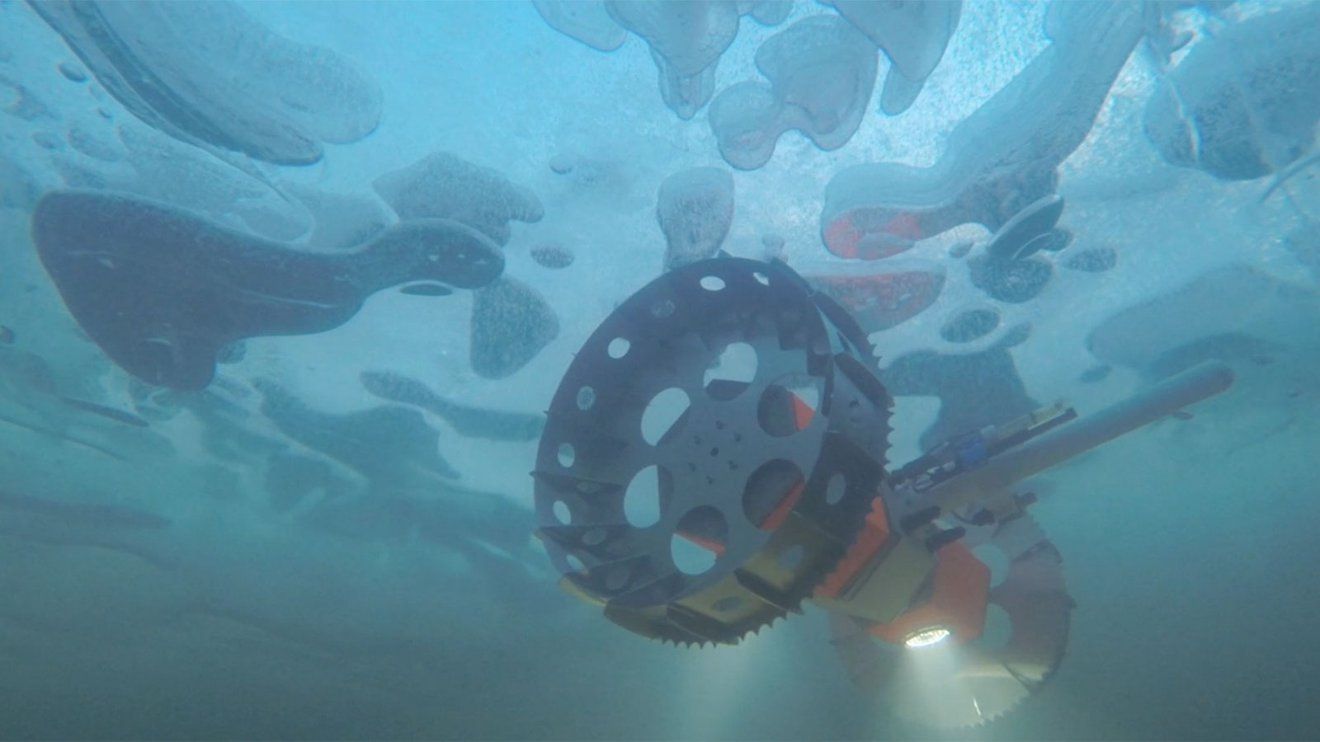
\includegraphics[width=10cm]{NASAbruie20191118.jpg}
\caption{NASA BRUIE under-surface rover designed to explore alien oceans.\cite{NASA19} Image used for educational purposes in accordance with NASA Media Usage Guidelines \cite{NASA22}}
\label{fig:NASAbruie20191118}
\end{figure}

\begin{figure} [h]

     \centering
     \begin{subfigure} %{0.3\textwidth}
     \centering
         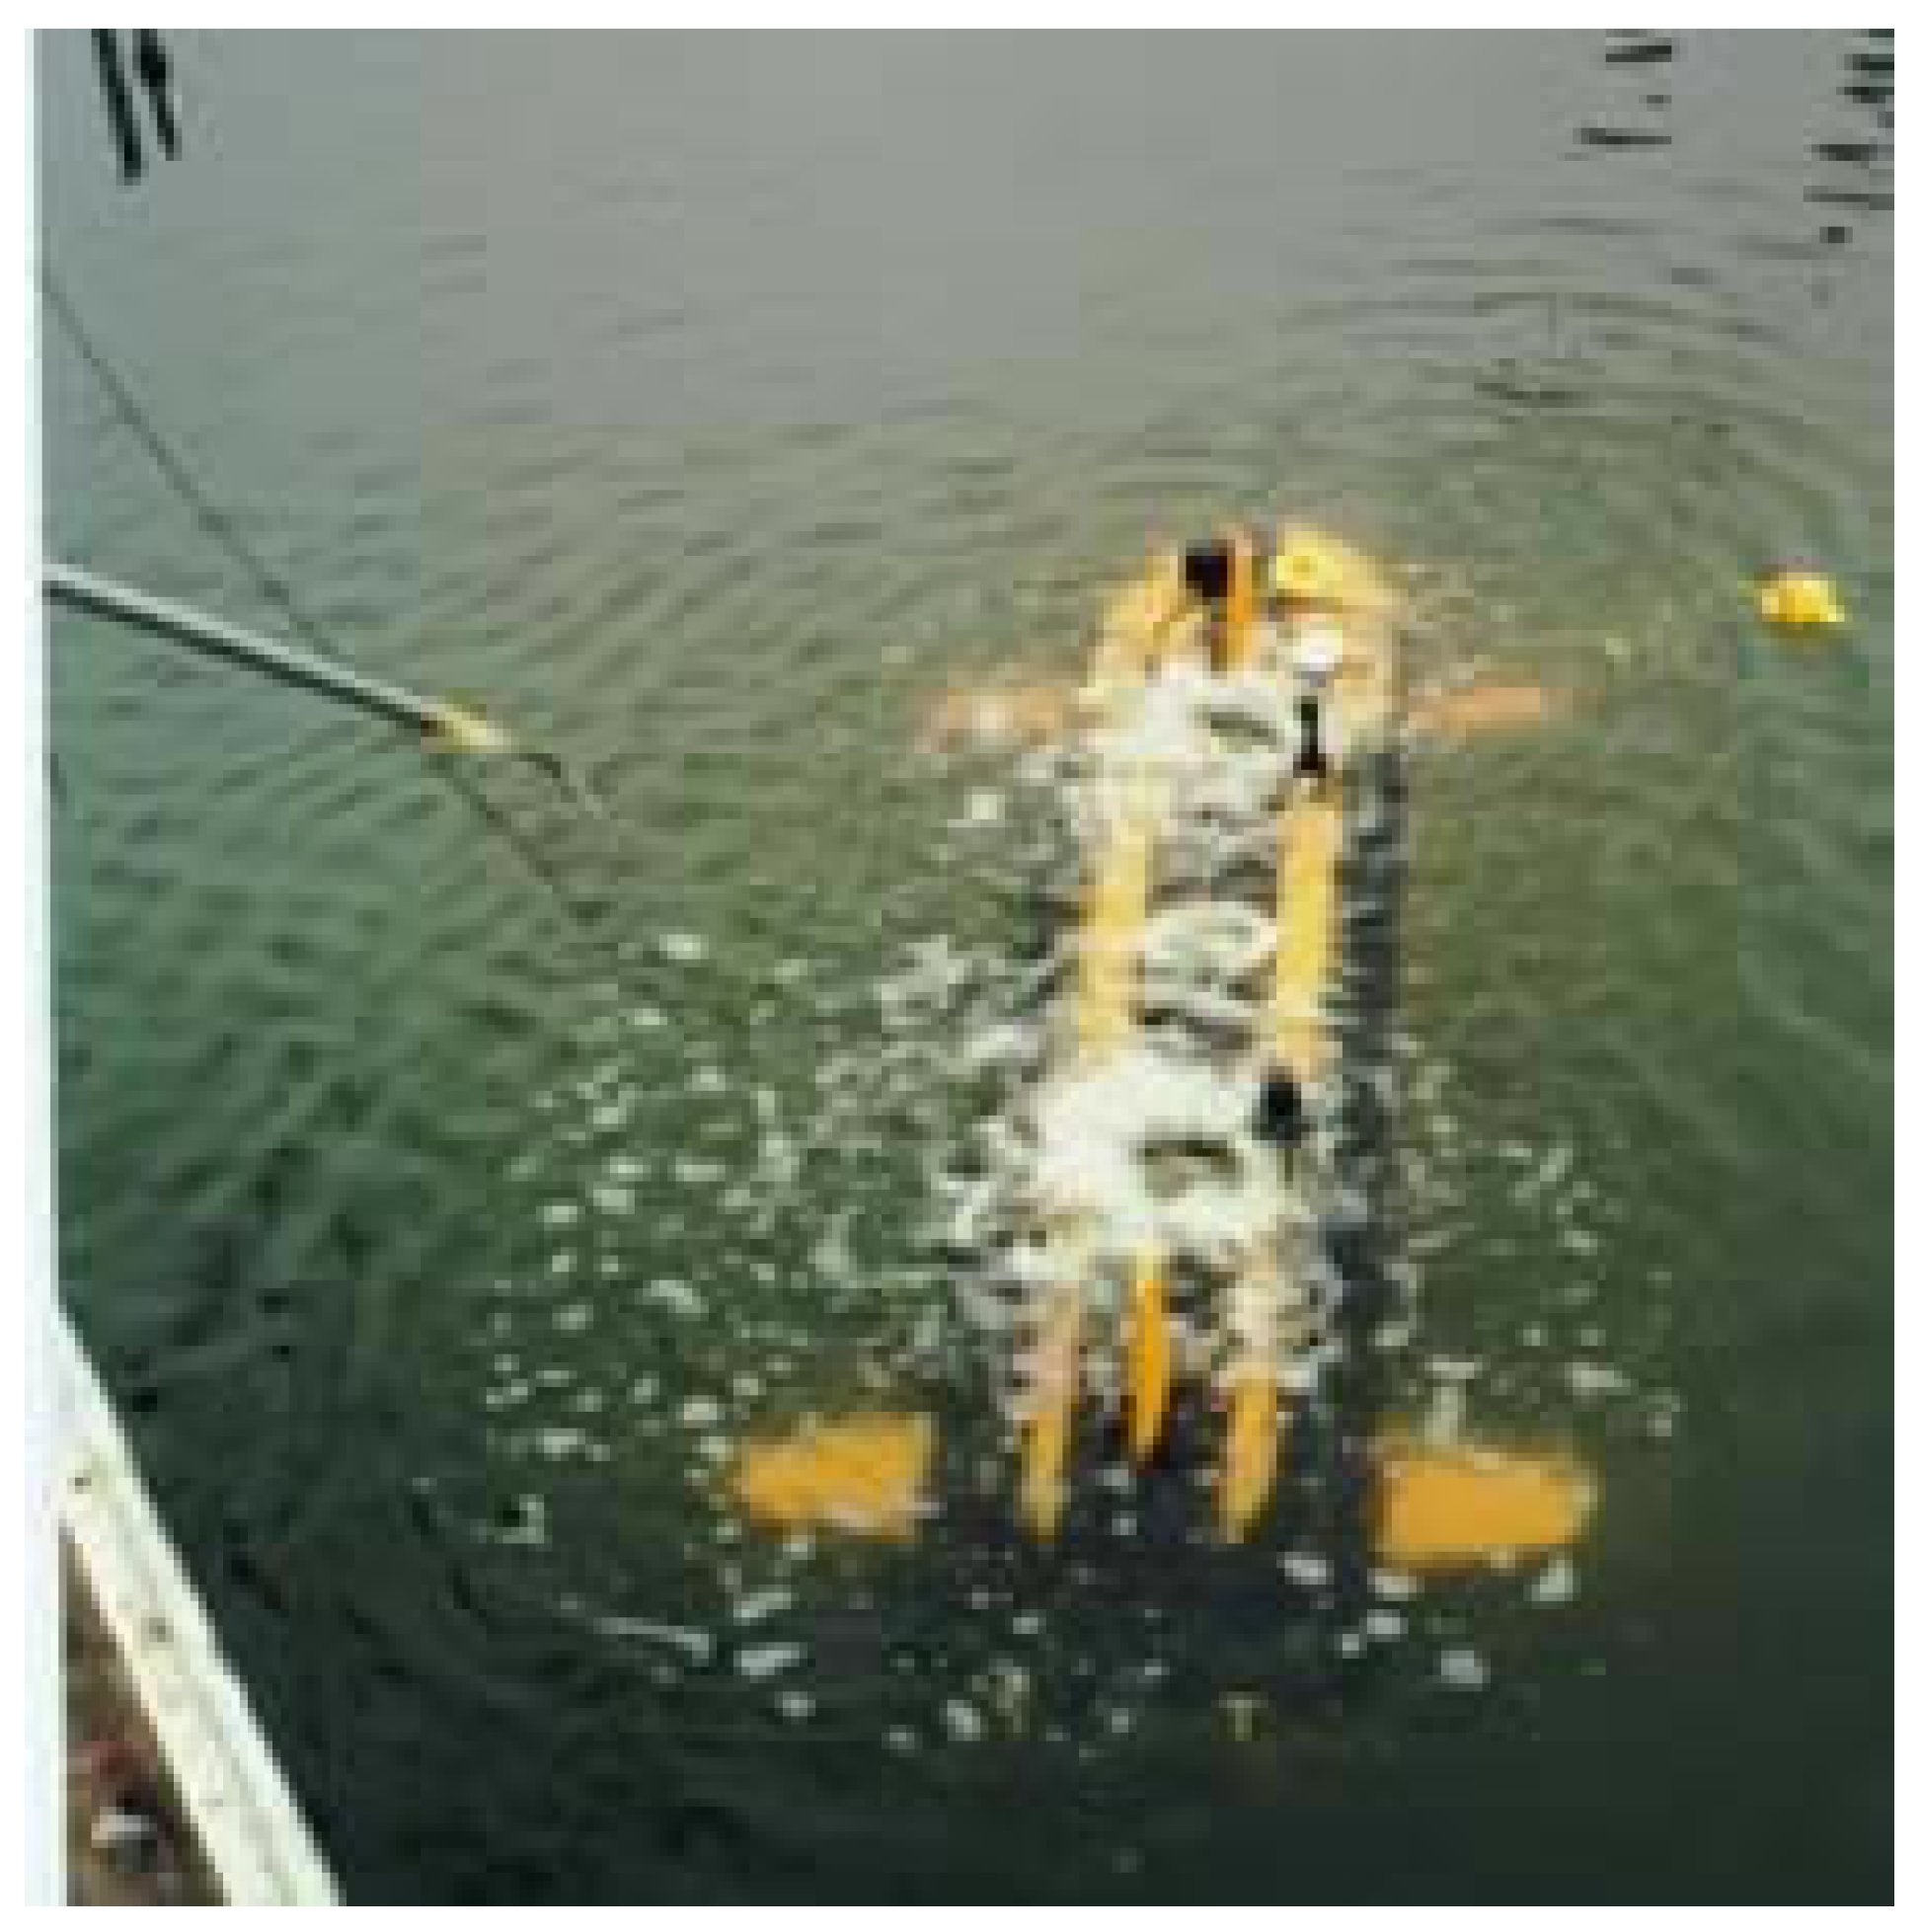
\includegraphics[width=3.5cm]{Phoenix.png} 
         %\caption{$(a)$}
      \label{fig:Phoenix}
     \end{subfigure}
     \hfill
     \begin{subfigure}%{(b)\textwidth}
         \centering
         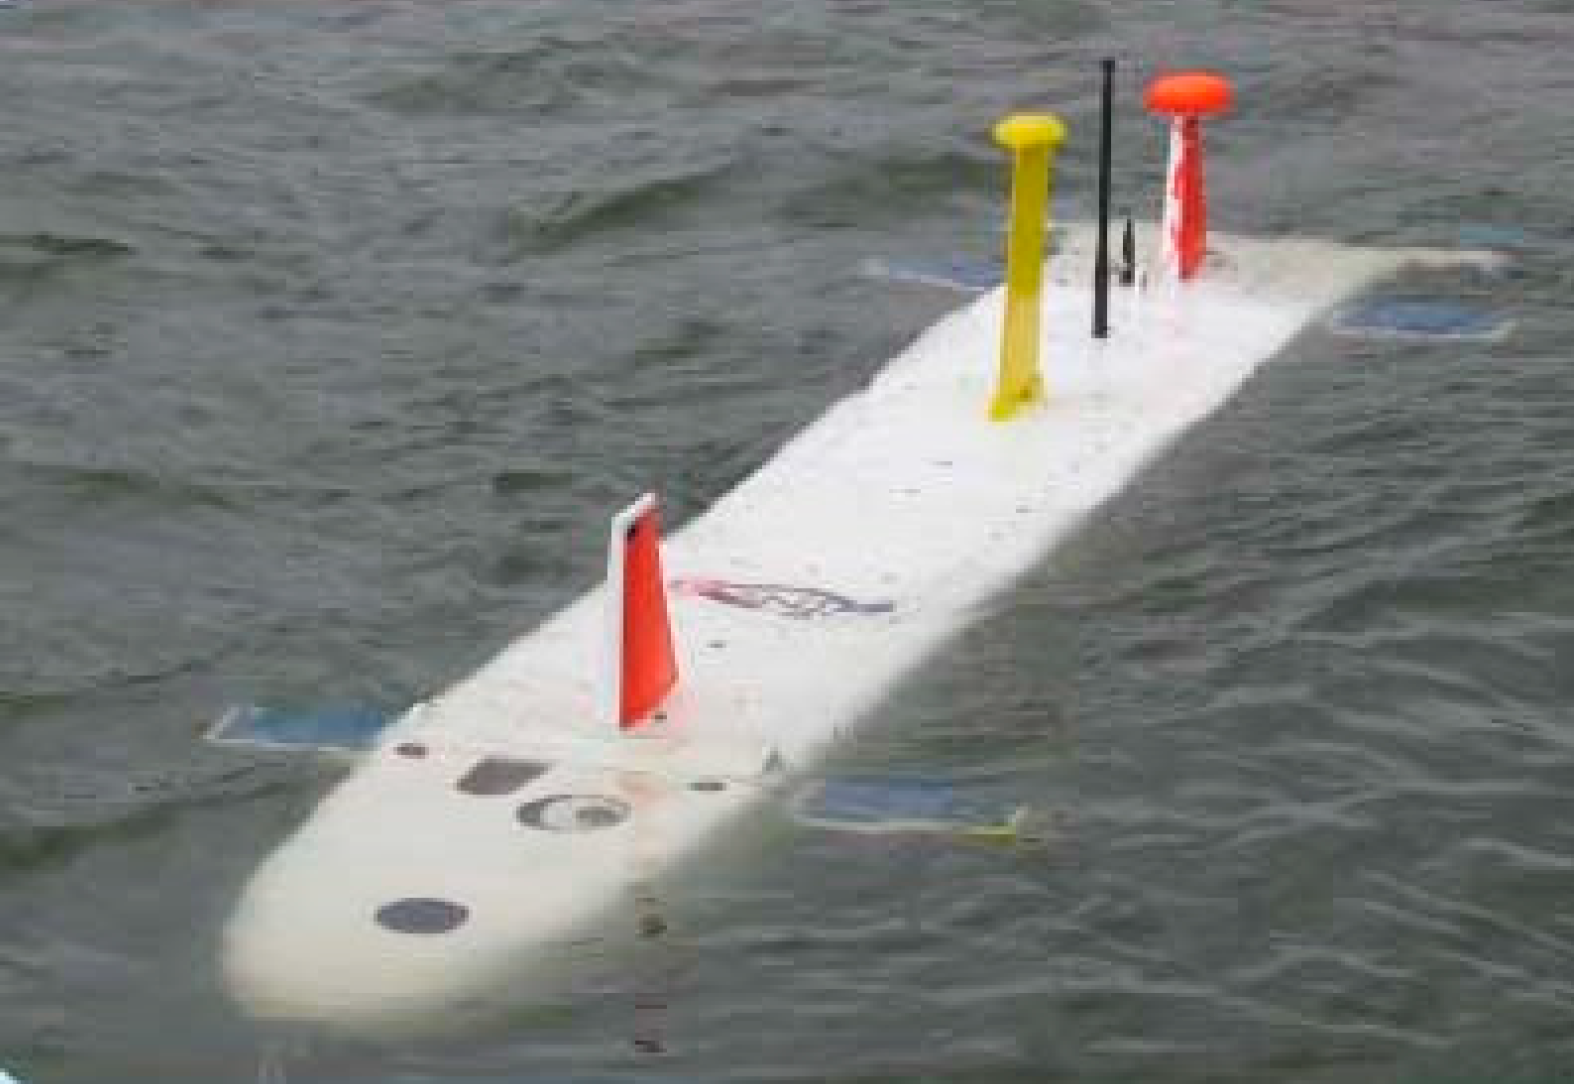
\includegraphics[width=5cm]{aries .png}
         \label{fig:Phoenix}
     \end{subfigure}
     \hfill
     \begin{subfigure}%{(c)\textwidth}
         \centering
         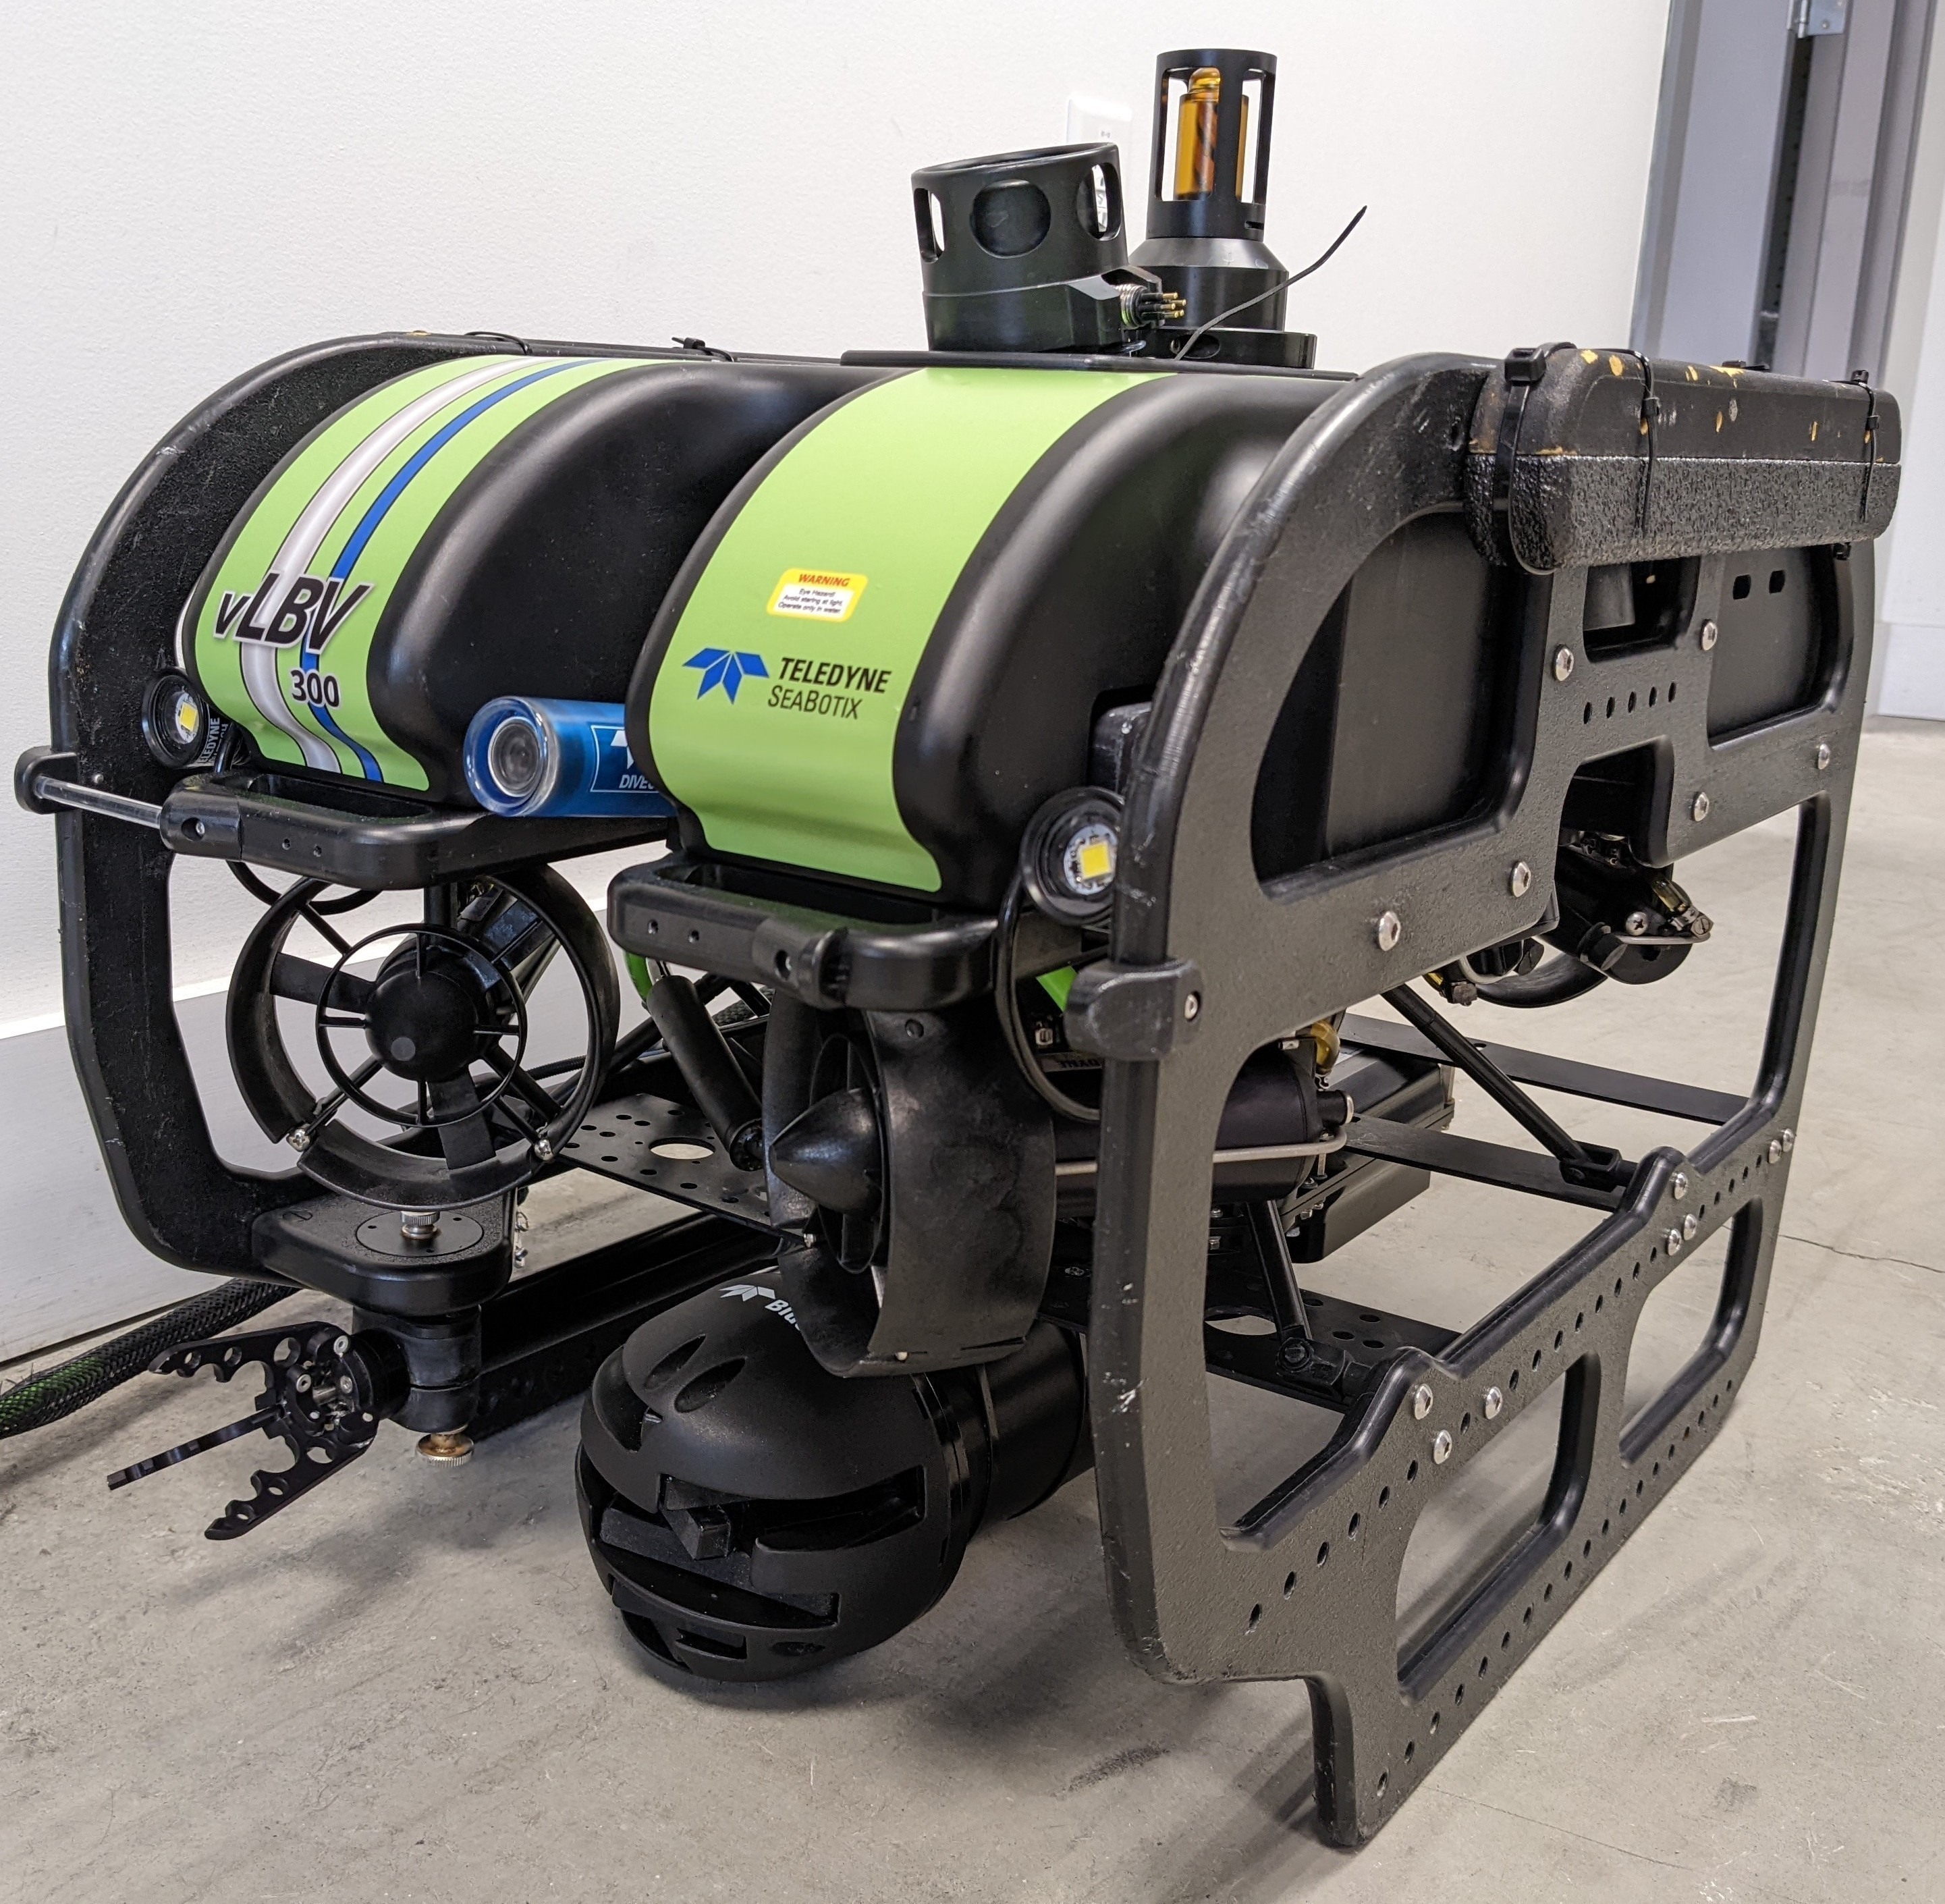
\includegraphics[width=3.5cm]{vlbv_002_crop.jpg}
         \label{fig:Phoenix}
     \end{subfigure}
        \caption{Remotely and autonomously operated undersea vehicles used to develop the methods proposed in this research: (a) Naval Postgraduate School Phoenix autonomous unmanned underwater vehicle \cite{Sands20} originally taken from \cite{NPS22}, (b) Naval Postgraduate School Aries autonomous unmanned underwater vehicle \cite{Sands18} originally taken from \cite{NPS22}, where image may be distributed or copied, subject only to any indicated copyright restrictions and normally accepted procedures for properly crediting sources as done here.\cite{NPSCopy22}, and (c) Seabotix vLBV 300 remotely operated submersible. Photo taken in lab.}
        \label{fig:three graphs}
\end{figure}

\subsection{Proposed innovations} 

This section succinctly and directly lists the innovations presented in this manuscript.

%Numbered lists can be added as follows:
\begin{enumerate}
\item	First-time development and presentation of deterministic artificial intelligence applied to yaw control of remotely piloted submersible (the Seabotix vLBV 300 in this case): includes both self-awareness statements and newly presented parameterization of optimal learning. 
\item	First instantiation of cubic polynomial autonomous trajectory generation supplied to deterministic self-awareness statements;
\item	Illustration of milli-degree tracking accuracy on the very first heading change of an aggressive shaped-square wave command, and an additional sixty percent (root mean square) error reduction by the third heading change of the square wave (illustrating the efficacy of optimal learning to eliminate startup transient behavior).
\end{enumerate}

\subsection{Manuscript structure} 
The next section describes the methods and materials used in the manuscript with the results of validating simulation experiments provided next in section 3 followed by a very brief discussion of the results and how they can be interpreted from the perspective of previous studies and of the working hypotheses. The findings and their implications are discussed in the broadest context possible. Future research directions are also highlighted.

%%%%%%%%%%%%%%%%%%%%%%%%%%%%%%%%%%%%%%%%%%
\section{Materials and Methods}
This section builds the proposed methodology from first principles cited in the Introduction, naturally starting with the system dynamics which lead to the governing differential equations of motion, which are quickly re-parameterized to permit two-norm optimal feedback learning. Since utilization of the governing equations necessitates expression of a desired trajectory (and that expression is preferably autonomous and analytic), autonomous trajectory generation is introduced next, where cubic polynomials are introduced and proposed. These notions are assembled (as depicted in \ref{fig:DAItopology}) to produce control and resulting motion trajectories where results are presented in section 3 and discussed in section 4. The presentation of materials and methods is described with sufficient details to allow others to replicate and build on published results, where the simulations used to manifest the mathematical developments in this section are presented in the Appendix, permitting readers to develop identical simulations themselves.

\subsection{Controller Architecture} 

\begin{figure}[h]
  \widefigure
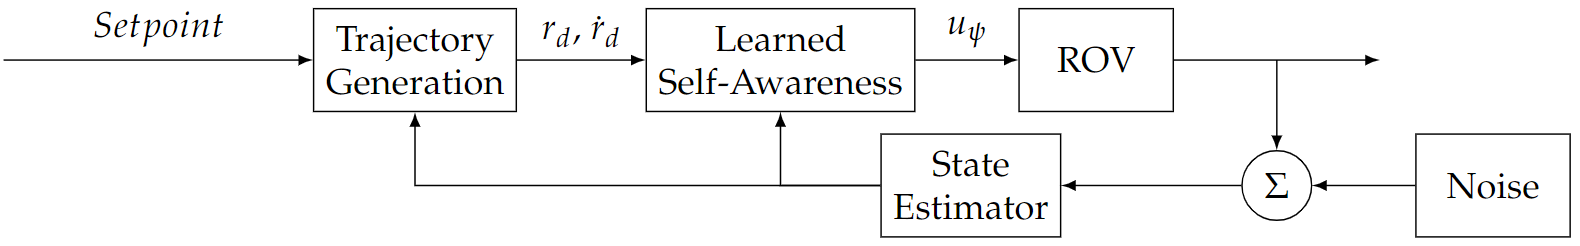
\includegraphics[width=13.5cm]{DAItopology.png}
\caption{Deterministic artificial intelligence topology}
\label{fig:DAItopology}
\end{figure}

The controller operations for a given time step are as follows. First, a trajectory is generated between the current system state and the set point. This trajectory is used to determine the current desired velocity and acceleration. Based on a system dynamics model the desired velocity and acceleration are used to calculate a control input to the system that will achieve the desired velocity and acceleration. The inputs are applied to the system, and then measurements of the system state are fed into a state estimator, and the estimated system state is used to optimally update the estimates for the parameters of the system dynamics model. Then this new system state estimate is used to generate a new trajectory, and the process repeats.

\subsection{System Dynamics}
The ROV yaw dynamics model asserted for this controller ignores Coriolis forces and assumes decoupled motion for calculating drag forces, and takes the form of equation (1) with variable definitions given in Table \ref{tab:variables}. In order to estimate the coefficients, equation \eqref{eq:psi_dynamics} must be rewritten in ``regression form'' i.e. in the form $y = \Phi\Theta$, where $\Phi$ is a matrix of known quantities and $\Theta$ is a vector the coefficients to estimate. This can be done by parameterizing the system in accordance with equation \eqref{eq:phi}.

\end{paracol}
\nointerlineskip
\begin{equation}
  \label{eq:psi_dynamics}
  \begin{aligned}
   A_0u_{\psi} =  &N_{\dot{w}}\dot{w} - r(N_r + N_{rr}|r|) - \dot{p}(I_{zx} - N_{\dot{p}}) - \dot{q}(I_{zy} - N_{\dot{q}}) - \sin(\theta)(gg_ym - Vb_yg\rho) + \dot{u}(N_{\dot{u}} - g_ym) + \\
    &\dot{v}(N_{\dot{v}} + g_xm) + \dot{r}(I_z + N_{\dot{r}}) - \cos(\theta)\sin(\phi)(gg_xm - Vb_xg\rho)
  \end{aligned}
\end{equation}
\linenumbers

\begin{table}[h]
  \begin{center}
    \begin{tabular}{|c|c| } 
      \hline
      Variable & Description \\
      \hline
      $u$, $v$, $w$, $p$, $q$, $r$ & Body frame x, y, z, roll, pitch, and yaw velocities  \\
      \hline
      $\phi$, $\theta$, $\psi$ & Inertial frame roll, pitch and yaw\\
      \hline
      $u_\psi$ & Yaw control input \\
      \hline
      $A_0$ & Coefficient relating $u_\psi$ to yaw torque\\
      \hline         
      $N_{\dot{u}}$, $N_{\dot{v}}$, $N_{\dot{w}}$, $N_{\dot{p}}$, $N_{\dot{q}}$, $N_{\dot{r}}$ & Added mass coefficients \\
      \hline
      $N_r$, $N_{rr}$ & Linear and nonlinear damping coefficient \\
      \hline
      $I_z$, $I_{zx}$, $I_{zy}$ & Moments of inertia\\
      \hline
      $g_x$, $g_y$, $g_z$ & Coordinates of the center of mass\\
      \hline
      $b_x$, $b_y$, $b_z$ & Coordinates of the center of buoyancy\\
      \hline
      $m$ & Vehicle mass\\
      \hline
      $g$ & Acceleration of gravity\\
      \hline
      $V$ & Vehicle volume\\
      \hline
      $\rho$ & Water density\\
      \hline      
    \end{tabular}
  \end{center}
  \caption{\label{tab:variables}Variable definitions.}
\end{table}

\nointerlineskip
\begin{equation}
  \label{eq:phi}
  \Phi^T =
  \begin{bmatrix} &
-\dot{p}\\ & \dot{p}\\ & -\dot{q}\\ & \dot{q}\\ & \dot{r}\\ & \dot{r}\\ & \dot{u}\\ & \dot{v}\\ & \dot{w}\\ & (-g\sin(\theta) - \dot{u})\\ & (\dot{v} - g\cos(\theta)\sin(\phi))\\ & g\sin(\theta)\\ & g\cos(\theta)\sin(\phi)\\ & -r\\ & -|r|r
  \end{bmatrix}
&   \quad \quad \Theta = \begin{bmatrix} &
    I_{zx}\\ & N_{\dot{p}}\\ & I_{zy}\\ & N_{\dot{q}}\\ & I_z\\ & N_{\dot{r}}\\ & N_{\dot{u}}\\ & N_{\dot{v}}\\ & N_{\dot{w}}\\ & g_ym\\ & g_xm\\ & Vb_y\rho\\ & Vb_x\rho\\ & N_r\\ & N_{rr}
  \end{bmatrix}
\end{equation}

\begin{paracol}{2}
\linenumbers
\switchcolumn
Then the optimal estimates for $\Theta$, $\hat{\Theta}$, can be computed using recursive least squares (RLS) as follows in equation \ref{eq:rls} \cite{astrom08} (which identically form the basis of comparative benchmark adaptive techniques \cite{Sands17}), and the readers will recognize equation \ref{eq:rls} as the feedback portion of the classical linear-optimal state estimator, the Kalman Filter \cite{Kalman60} - \cite{Kalman61}. Thus, deterministic artificial intelligence is akin a dual representation of a Kalman Filter applied to control rather than state estimation, where the limitation of linear or linearized feedforward is released and replaced with any form of coupled, nonlinear dynamics demanded by the governing physics. 
\begin{linenomath}
\begin{equation}
  \label{eq:rls}
  \begin{aligned}
    \hat{\Theta}(t) &= \hat{\Theta}(t - 1) + K(t)(\tau(t) - \Phi^T(t)\hat{\Theta}(t - 1)\\
    K(t) &= P(t)\Phi(t) = P(t - 1)\Phi(t)(I + \Phi^T(t)P(t - 1)\Phi(t))^{-1}\\
    P(t) &= (I - K(t)\Phi^T(t))P(t - 1)
  \end{aligned}
\end{equation}
\end{linenomath}

\subsection{State Estimation}
Estimates of the system states in $\Phi$ are required in order to estimate the parameters in $\Theta$. The simulator used to test the system provides ``truth'' measurements for roll, pitch, yaw, and their respective velocities, so those values are used directly. A Kalman filter is used to estimate the attitude accelerations. Since ``true'' measurements are used as the inputs to the Kalman filter and to the RLS estimation, this paper does not attempt to assess the performance of the controller in the presence of noisy measurements.

\subsection{Trajectory Generation}
The DAI based controller requires a trajectory to track between the current state and the desired state. It is desirable that the trajectory be continuous with the system velocity and position, and needs to reach the desired position and velocity after some finite time interval, i.e. if the current position is $x_0$, the final position is $x_f$, and the desired time to complete the move is $T$ then the trajectory $q(t)$ must satisfy
\begin{linenomath}
\begin{align}
  q(0) &= x_0, \;
  \dot{q}(0) = \dot{x}_0 \\  
  q(T) &= x_f, \;
  \dot{q}(T) = \dot{x}_f
\end{align}
\end{linenomath}
One way of satisfying these requirements is to choose a trajectory that is a cubic polynomial of the form
\begin{linenomath}
\begin{equation}
  \label{eq:q(t)}
  q(t) =  x_0 + \Delta x(at^3 + bt^2 + ct + d)
\end{equation}
\end{linenomath}
where $\Delta x = x_f - x_0$. Solving for the coefficients gives
\begin{linenomath}
\begin{align}
  a &= (\dot{x}_f - \frac{2\Delta x}{T} + \dot{x}_0)(\Delta xT^2)^{-1}\\
  b &= (\Delta x - \Delta xaT^3 - \dot{x}_0)(\Delta xT^2)^{-1}\\
  c &= \frac{\dot{x}_0}{\Delta x} \\
  d &= 0
\end{align}
\end{linenomath}
If constant velocity is assumed for  $t < t_0$ and $t > t_0 + T$ then the trajectory becomes the piecewise defined functions
\begin{linenomath}
\begin{align}
  q(t) &=
  \begin{cases}
    \dot{x}_0(t - t_0) + x_0 & t < t_0\\
    x_0 + \Delta x(a(t - t_0)^3 + b(t - t_0)^2 + c(t - t_0) + d) & t_0 \leq t \leq t_0 + T\\
    \dot{x}_f(t - t_0 - T) + x_f & t > t_0 + T
  \end{cases} \label{eq:q}\\
  \dot{q}(t) &=
  \begin{cases}
    \dot{x}_0 & t < t_0\\
    \Delta x(3a(t - t_0)^2 + 2b(t - t_0) + c) & t_0 \leq t \leq t_0 + T\\
    \dot{x}_f& t > t_0 + T
  \end{cases} \label{eq:q_dot}\\
  \ddot{q}(t) &=
  \begin{cases}
    0 & t < t_0\\
    \Delta x(6a(t - t_0) + 2b)  & t_0 \leq t \leq t_0 + T\\
    0 & t > t_0 + T
  \end{cases} \label{eq:q_ddot}\\   
\end{align}
\end{linenomath}
\subsection{Control Output}
Each time the user specified yaw set point changes a new ``primary'' trajectory, $q_1(t)$, is generated between the current vehicle state, and the specified set point and 0 velocity. Then, on each time step, a ``secondary'' trajectory $q_2(t)$ is generated between the current vehicle position, and the position and velocity of the primary trajectory a short time, $\Delta t$, in the future. i.e. if the current position and velocity at time $t_k$ are $x_k$ and $\dot{x}_k$, then the ``secondary'' trajectory, $q_2(t)$, is generated between  $x_k$ and $\dot{x}_k$, and $q_1(t_k + \Delta t)$ and $\dot{q}_1(t_k + \Delta t)$. This keeps the vehicle on the specified ``primary'' trajectory, driving it back to the trajectory if it is perturbed. The $\Delta t$ used to generate the ``secondary'' trajectory is a tunable parameter. For the system simulated in this paper a value of 0.25 seconds was chosen.

The velocity and acceleration trajectories calculated for $q_2(t)$ using equations \eqref{eq:q_dot} and \eqref{eq:q_ddot}, and the estimated model parameters calculated from \eqref{eq:rls} are then used to calculate the controller output for each time step. First calculate the desired yaw velocity, $r_d$, from equation \eqref{eq:q_dot}, then calculate the desired yaw acceleration, $\dot{r}_d$, from equation \eqref{eq:q_ddot}. Next, substitute $r_d$ and $\dot{r}_d$ for $r$ and $\dot{r}$ respectively in $\Phi$ to yield the desired state vector $\Phi_d$. Then using the most recent estimate for the model parameters $\hat{\Theta}$ calculated from \eqref{eq:rls} the prescribed yaw torque is
\begin{linenomath}
\begin{equation}
  \label{eq:ctrl_output}
  \tau_d = \Phi_d\hat{\Theta}  
\end{equation}
\end{linenomath}
And finally the yaw torque is related to the control, $u_\psi$, by the $A_0$ coefficient via
\begin{linenomath}
\begin{equation}
  u_{psi} = \frac{\tau_d}{A_0} 
\end{equation}
\end{linenomath} 

%%%%%%%%%%%%%%%%%%%%%%%%%%%%%%%%%%%%%%%%%%
\section{Results}

This section provides a concise and precise description of the experimental simulation results, their interpretation as well as the experimental conclusions that can be drawn.

The controller was tested by applying a series of positive then negative 30 degree step changes to the desired vehicle heading. The trajectory generation was configured to generate a trajectory that would take approximately 2.42 seconds to complete the 30 degree heading change. Figure \ref{fig:dai_step} shows the response to these inputs and Table \ref{tab:results} summarizes some performance metrics. The rise time in the table is calculated as the amount of time to complete 99.9\% of the thirty degree heading change (29.97 degrees). The settling time is calculated as the amount of time required after the heading change was started before the heading stayed within 0.1\% (.03 degrees) of the final value.

\begin{figure}[h]
\centering
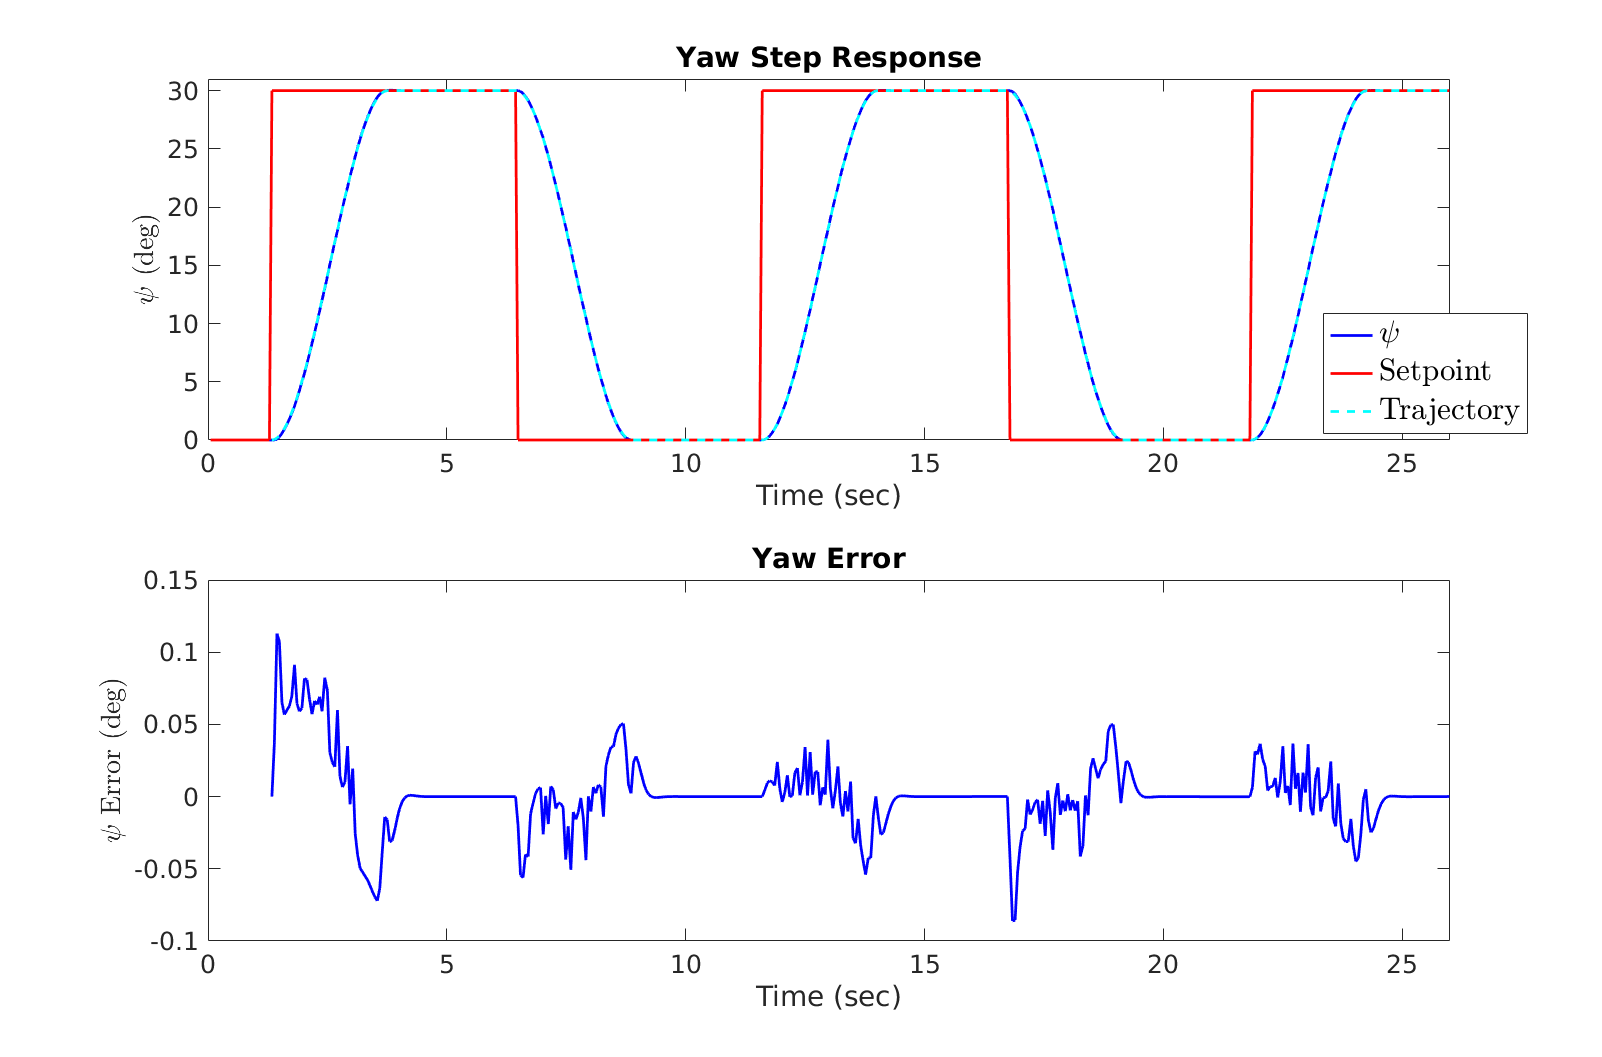
\includegraphics[width=15cm,inner]{dai_step.png}
\caption{Yaw step response and the associated trajectory tracking error \label{fig:dai_step}}
\end{figure}

Deterministic artificial intelligence was able to quickly converge to values that provided a stable response with good tracking of the desired trajectory. Even for the first heading change the controller was able to closely track the trajectory, with a root mean square (RMS) tracking error of only .043 degrees. By the third positive step the RMS error had further decreased by almost a factor of 3, to only .016 degrees.

The simulator was configured such that there were no disturbances, and such that the measurements obtained from the simulator were not corrupted by noise. This represents idealized conditions, but serves to validate that the general algorithm and controller architecture may be viable.

\begin{table}[ht]
  \begin{center}
    \begin{tabular}{|c|c|c|c|c| } 
      \hline
      & Rise Time (sec) & Settling Time (sec) & Overshoot (deg)  & Error (RMS deg) \\
      \hline
      \textbf{First Step} & 2.362 & 2.608 & \hl{0.104} & \hl{0.0426} \\
      \hline
      \textbf{Third Step} & 2.413 & 2.425 & \hl{0.083} & \hl{0.0164} \\
      \hline  
    \end{tabular}
  \end{center}
  \caption{\label{tab:results}Response performance for the first and third positive 30 degree heading changes.}
\end{table}

%%%%%%%%%%%%%%%%%%%%%%%%%%%%%%%%%%%%%%%%%%
\section{Discussion}

The slight variations in response for each step, best seen in the slightly differing amounts of error in Figure \ref{fig:dai_step}, are likely the result of small variations in the model parameters and timing variations in the controller and/or simulator.

Previous applications of DAI to attitude control and UUVs have demonstrated that DAI can be used to achieve a high degree of trajectory tracking accuracy with minimal lag \cite{Sands20, Smeresky20}. This paper presents a DAI based controller that uses a different feedback mechanism and trajectory generation scheme; however, the results achieved by the DAI controller in this paper are consistent with the level of performance achieved by the previous DAI controllers. The results are also consistent with the central hypothesis behind DAI: that using a system's own dynamics as the control law can produce extremely effective trajectory tracking.

\subsection{Findings and their implications}
The controller plays a crucial part in the operation of an ROV. At its core, the controller's role is to translate the operator's instructions into actual vehicle motion, so the operator's ability to complete an objective is directly tied to the quality of the ROV's controller. The controller outlined in this paper provides a framework that presents a number of advantages to both operators and manufacturers over classical controllers typically used for ROV control. One advantage that this controller presents is the high degree of tracking accuracy. The controller presented here achieved milli-degree tracking accuracy within seconds of startup. This level of accuracy makes the controller well suited to extremely sensitive tasks which require a high degree of precision such as sampling delicate marine life or explosive ordnance disposal (EOD). The adaptive nature of the controller also makes it well suited to applications where the system dynamics may change unexpectedly. Again, EOD operations present situations where the ROV may be subject to significant damage, and the adaption could allow recovery and mission completion after sustaining damage that would otherwise cripple the vehicle. The adaptive nature of the controller also means that it required no tuning. Tuning can be an expensive part of ROV design, often requiring significant time from trained engineers. Removing the requirement for tuning presents manufacturers with an opportunity to reduce the cost to produce an ROV.

The approach is validated to effectively control the remotely operated vehicle with increasing accuracy with the passage of time. The application of deterministic artificial intelligence in autonomous unmanned vehicles (UUVs) proved to be effective with no design tuning required, and that feature appears to be true for the disparate system equations of the Seabotix vLBV 300 remotely operated vehicle. The working hypothesis is proved by results that are comparable to the previous studies on UUVs. 

\subsection{Recommendations for future research}
This manuscript proposed a controller architecture and tested it for yaw control of an ROV under idealized conditions, namely no disturbances and perfect measurements. This presents many avenues for future work. One area of future work involves expanding the controller testing and validation with the end goal of a control system operating in real-world open ocean conditions. The first step in this is to apply the controller to the ROV's other degrees of freedom: roll, pitch, position and depth. Then performance of these controllers will be assessed under simulated conditions more akin to a real-world operating environment. This will involve adding measurement noise and disturbances such as wind, swell or tether dynamics to the simulated test environment. After demonstrating performance under non-ideal simulated conditions the research will progress to laboratory validation on real vehicle hardware, and finally to assessing the performance of the proposed controller on a "live" ROV in open water conditions. 

Another area of future work involves assessing and improving the control architecture itself. The controller's adaptive nature will be tested to determine the controller's robustness to changes in system dynamics, for example from damage to the vehicle or changes in payloads. Alternate trajectory generation schemes will also be explored. These will focus on optimal trajectories that for example minimize energy consumption; and trajectories generated under constraints such as maximum and minimum applied force, or maximum slew rate of actuators that better reflect the actual operating capabilities of the ROV. Previous work such as \cite{Smeresky20} has evaluated the efficacy of DAI based controllers against "classic" controllers, but an important area of future research will involve comparing this DAI controller against controllers based on other forms of artificial intelligence such as deep learning. Finally, analysis of the computational burden required for this controller should be performed in order to determine minimum required system specifications.

The cited lineage (e.g. Chasle, Slotine, Fossen, Nakatani, Cooper, Smeresky, etc.) develops dynamic-based controls in order to instill inherent resilience to dynamic parameter change, and sources of such change include damage, fuel expenditure, and sudden grasping of objects by the remotely operated vehicle. Following this prequel research, the limits of efficacy of the validated approach should be investigated to ascertain the ability to autonomously reject the deleterious effects of such changes. Next, bench-board laboratory experiments should be performed to prepare for validating hardware experiments in the open ocean. 

%%%%%%%%%%%%%%%%%%%%%%%%%%%%%%%%%%%%%%%%%%
%%%%%%%%%%%%%%%%%%%%%%%%%%%%%%%%%%%%%%%%%%

%%%%%%%%%%%%%%%%%%%%%%%%%%%%%%%%%%%%%%%%%%
\authorcontributions{ Conceptualization, S.O. and T.S.; methodology, S.O. and T.S.; software, S.O.; validation, S.O. and T.S.; formal analysis, S.O.; investigation, S.O. and T.S.; resources, T.S.; writing---original draft preparation, S.O. and T.S.; writing---review and editing, S.O. and T.S.; visualization, S.O. and T.S.; supervision, T.S.; project administration, S.O. and T.S.; funding acquisition, T.S. All authors have read and agreed to the published version of the manuscript. Please turn to the  \href{http://img.mdpi.org/data/contributor-role-instruction.pdf}{CRediT taxonomy} for the term explanation. Authorship must be limited to those who have contributed substantially to the work~reported.} 

\funding{This research received no external funding}

\dataavailability{For access to archived datasets analyzed or generated during the study, please contact the corresponding author.} 

\end{paracol}

%%%%%%%%%%%%%%%%%%%%%%%%%%%%%%%%%%%%%%%%%%
\vspace{6pt} 

%%%%%%%%%%%%%%%%%%%%%%%%%%%%%%%%%%%%%%%%%%

\pagebreak

%%%%%%%%%%%%%%%%%%%%%%%%%%%%%%%%%%%%%%%%%%
%% Optional
\appendixtitles{yes} % Leave argument "no" if all appendix headings stay EMPTY (then no dot is printed after "Appendix A"). If the appendix sections contain a heading then change the argument to "yes".
\appendixstart
\appendix
\section{MATLAB Code}
\subsection{dai\_analysis.m}
\begin{lstlisting}[language=Matlab]
  %% 
  clc
  clear
  close all

  %% Load
  log = '20220128002145_10x_psi_step_30';
  load(['scripts/' log '/' log '_ADAPTIVE_CTRL_STAT.mat']);

  %% Analyze
  t = UNIX_timestamp - UNIX_timestamp(1);
  t_start = 0;
  t_end = 26;
  to_use = t > t_start & t < t_end;
  t = t(to_use);
  psi = polar_correct(PSI(to_use), -180, 180);
  psi_dot = PSI_DOT(to_use);
  psi_trajectory = polar_correct(PSI_TRAJ(to_use), -180, 180);
  setpoint = polar_correct(UC(to_use), -180, 180);

  %% stats for first/last steps
  first_start = 1.25;
  first_end = 6;
  first_step = t > first_start & t < first_end;
  first_step_info = stepinfo(psi(first_step), t(first_step) - first_start, 'RiseTimeLimits', [0, .999], 'SettlingTimeThreshold', .001)
  first_traj = psi_trajectory(first_step);
  first_traj(1) = 0;
  first_psi = psi(first_step);
  first_error = first_traj - first_psi;
  first_rms_error = sqrt(mean(first_error .^2))
  first_max_error = max(abs(first_error))

  last_start = 21.8;
  last_end = 26;
  last_step = t > last_start & t < last_end;
  last_step_info = stepinfo(psi(last_step), t(last_step) - last_start, 'RiseTimeLimits', [0, .999], 'SettlingTimeThreshold', .001)
  last_traj = psi_trajectory(last_step);
  last_psi = psi(last_step);
  last_error = last_traj - last_psi;
  last_rms_error = sqrt(mean(last_error .^2))
  last_max_error = max(abs(last_error))
  %% Plots
  label_fontsize = 24;
  axis_fontsize = 18;
  linewidth = 1.25;
  ax = [t_start t_end 0 31];

  % Plot step response
  figure
  subplot(2, 1, 1)
  plot(t, psi, 'blue', 'linewidth', 2)
  title 'Yaw Step Response'
  ylabel('$\psi$ (deg)', 'Interpreter', 'Latex', 'FontSize', axis_fontsize)
  xlabel('Time (sec)')
  hold on
  plot(t, setpoint, 'red', 'linewidth', 2)
  plot(t, psi_trajectory, '--c', 'linewidth', 2)
  legend({'$\psi$', 'Setpoint', 'Trajectory'}, 'Interpreter', 'latex', 'FontSize', 22);
  set(gca,'FontSize', axis_fontsize)
  axis(ax);

  % Plot error
  subplot(2, 1, 2)
  plot(t, psi_trajectory - psi,  'blue', 'linewidth', 2);
  title 'Yaw Error'
  ylabel('$\psi$ Error (deg)', 'Interpreter', 'Latex');
  xlabel 'Time (sec)'
  set(gca,'FontSize', axis_fontsize)
  axis([t_start t_end -0.1 0.15])

  figure
  plot(psi, psi_dot)
  axis equal
  % axis square
\end{lstlisting}
\section{C++ Code}
\subsection{adaptive\_control.cpp}
\begin{lstlisting}[language=c++]
/**
 * @author Shay Osler
 */

#include <adaptive_control_version.h>
#include <indirect_self_tuning_regulator.h>
#include <dai.h>
#include <matrix_utils.h>
#include <state_estimator/state_estimator.h>
#include <trajectory.h>
#include <sinusoidal_trajectory.h>
#include <cubic_trajectory.h>
#include <SO_utils.h>

#include <sno/logger.h>
#include <sno/sno_macros.h>
#include <sno/time_utils.h>

#include <opencmd_defs.h>
#include <opensea/ops.h>
#include <opensea/gss_types/pcomms.h>
#include <opensea/gss_types/effort.h>
#include <opensea/gss_types/cmd.h>
#include <opensea/gss_types/nav_solution.h>

#include <lcm/lcm-cpp.hpp>
#include <atomic>
#include <chrono>
#include <thread>

///////////////////////////////////////////////////////////////////////
// Global Variables
///////////////////////////////////////////////////////////////////////
namespace
{
/**
 * @brief Publish/subscribe interface
 */
std::shared_ptr<gss::OPS> m_plcm;

/**
 * @brief Channel to subscribe to nav solutions
 */
std::string m_nav_channel = "OPENINS_NAV_SOLUTION";

/**
 * @brief Channel to subscribe to setpoints on
 */
std::string m_ctrl_cmd_channel = "OPENCMD_CMD";

/**
 * @brief Channel to subscribe to opencmd efforts on
 */
std::string m_effort_in_channel = "OPENCMD_EFFORT";

/**
 * @brief Channel to publish effort commands on
 */
std::string m_effort_out_channel = "ADAPTIVE_CTRL_EFFORT";

/**
 * @brief Controller status channel
 */
std::string m_status_channel = "ADAPTIVE_CTRL_STAT";

/**
 * @brief Command channel
 */
std::string m_cmd_channel = "ADAPTIVE_CTRL_CMD";

/**
 * @brief Main thread sleep interval, ms
 */
const std::chrono::milliseconds m_main_sleep_ms(50);

/**
 * @brief Last received efforts
 */
gss::types::Effort m_last_effort_rx;

/**
 * @brief Last transmitted efforts
 */
gss::types::Effort m_last_effort_tx;

/**
 * @brief Indirect self tuning regulator
 */
std::shared_ptr<ISTR> m_istr;

static const size_t L = 15; // Number of parameters being estimated
static const size_t N = 18; // Number of states
static const size_t M = 6;  // Control inputs

/**
 * @brief Deterministic artificial intelligence controller
 */
std::shared_ptr<DAI_controller<L, N, M>> m_dai;

/**
 * @brief True if autopilot is enabled
 */
bool m_enable_auto{false};

/**
 * @brief True if DAI controller should be enabled
 */
bool m_enable_dai{false};

/**
 * @brief True if closed loop control should be used with DAI. If false then
 * DAI will only be used as a feed forward controller
 */
bool m_enable_closed_loop_dai{false};

/**
 * @brief True if ISTR controller should be enabled
 */
bool m_enable_istr{false};

/**
 * @brief Current controller setpoint
 */
double m_setpoint{0};

/**
 * @brief Time when the control move should be finished
 */
double m_ctrl_tf{0};

/**
 * @brief Kalman filter for estimating angular accelerations
 */
State_estimator m_accel_estimator;

/**
 * @brief Current trajectory to follow
 */
std::shared_ptr<Trajectory> m_psi_trajectory;

/**
 * @brief Last received nav solution
 */
gss::types::Nav_solution m_last_soln;
}

///////////////////////////////////////////////////////////////////////
// Function Declarations
///////////////////////////////////////////////////////////////////////

/**
 * @brief Initialize the indirect self tuning regulator
 */
void Initialize_istr();

/**
 * @brief Run the indirect self tuning regulator
 * @param Received nav solution
 */
void Run_istr(const gss::types::Nav_solution* msg);

/**
 * @brief Initialize the deterministic artifical intelligence controller
 */
void Initialize_dai();

/**
 * @brief Callback function for when controller commands are received
 * @param buf Received LCM buffer
 * @param channel Channel the message was received on
 * @param msg Command message
 */
void On_ctrl_cmd_received(const gss::OPS::Receive_buffer&,
                     const std::string&,
                     const gss::types::Cmd* msg);

/**
 * @brief Callback function for when vehicle nav solutions are received
 * @param buf Received LCM buffer
 * @param channel Channel the message was received on
 * @param msg Command message
 */
void On_nav_received(const gss::OPS::Receive_buffer&,
                     const std::string&,
                     const gss::types::Nav_solution* msg);

/**
 * @brief Callback function for when effort commands are received
 * @param buf Received LCM buffer
 * @param channel Channel the message was received on
 * @param msg Command message
 */
void On_effort_received(const gss::OPS::Receive_buffer&,
                        const std::string&,
                        const gss::types::Effort* msg);

/**
 * @brief Generate a trajectory from the current position to the specified position
 * and velocity
 * @param xf Final Position
 * @param vf Final velocity
 * @return Trajectory
 */
std::shared_ptr<Trajectory> Generate_trajectory(const double xf,
                                                const double vf =0 );

///////////////////////////////////////////////////////////////////////
// Function Definitions
///////////////////////////////////////////////////////////////////////

void Initialize_istr()
{
  // Mark last received efforts as invalid
  m_last_effort_rx.time_unix_sec = -1;

  // Desired TF:
  //          0.1761q
  //  -----------------------
  //  (q^2 + 1.223q + 0.3743)

//  Eigen::Matrix<double, ISTR::N, 1> Am{1.223, 0.3743};
  Eigen::Matrix<double, ISTR::N, 1> Am{-1.3205, 0.4966};
  Eigen::Matrix<double, ISTR::M+1, 1> Bm{8.0186, 3.1818};
  double a0 = 0;
  Eigen::Matrix<double, ISTR::N+ISTR::M+1, 1> theta0{0, 0, .01, .2};
  Eigen::Matrix<double, ISTR::N+ISTR::M+1, ISTR::N+ISTR::M+1> P0{{100, 0, 0, 0},
                                                                 {0, 100, 0, 0},
                                                                 {0, 0,   1, 0},
                                                                 {0, 0,   0, 1}};
  m_istr = std::make_shared<ISTR>(Am, Bm, a0, theta0, P0);
}

///////////////////////////////////////////////////////////////////////

void Run_istr(const gss::nav_solution_t* msg)
{
  // Check that nav is valid
  if(!msg->attitude_ok)
  {
    return;
  }
  if(!m_istr)
  {
    return;
  }
  // run every nth time
  static size_t count = 0;
  if( (count++ % 1) != 0)
  {
    return;
  }

  // Get controller output
  double y = msg->attitude_dot[2];
  const auto [effort, theta_hat] = m_istr->Get_control_output(y,
                                                              m_setpoint,
                                                              m_last_effort_tx.effort_psi);

  {}
  // If we're in closed loop mode, publish
  if(m_enable_auto
     && m_enable_istr
     && m_last_effort_rx.time_unix_sec > 0)
  {
    gss::effort_t effort_cmd = m_last_effort_rx;
    double effort_out = effort;
    double max_effort = 50;
    double min_effort = -max_effort;
    if(effort_out > max_effort)
    {
      effort_out = max_effort;
    }
    else if(effort_out < min_effort)
    {
      effort_out = min_effort;
    }
    effort_cmd.effort_psi = effort_out;
    m_plcm->Publish(m_effort_out_channel, &effort_cmd);
    m_last_effort_tx = effort_cmd;
  }

  gss::pcomms_t stat;
  static uint32_t count_publish = 0;
  stat.time_unix_sec = so::Time_utils::Unix_time();
  stat.count_publish = count_publish++;
  stat.analogs.push_back({"A1", theta_hat[0]});
  stat.analogs.push_back({"A2", theta_hat[1]});
  stat.analogs.push_back({"B0", theta_hat[2]});
  stat.analogs.push_back({"B1", theta_hat[3]});
  stat.analogs.push_back({"UC", m_setpoint});
  stat.analogs.push_back({"U", effort});
  stat.analogs.push_back({"Y", y});
  stat.digitals.push_back({"AUTO_DEPTH_ENABLE", m_enable_auto});
  stat.num_analogs = stat.analogs.size();
  stat.num_digitals = stat.digitals.size();
  stat.num_messages = stat.messages.size();
  m_plcm->Publish(m_status_channel, &stat);
}

///////////////////////////////////////////////////////////////////////

void Initialize_dai()
{
  // Initialize acceleration estimator
  m_accel_estimator.Initialize(so::Time_utils::Unix_time(),
                               State_estimator::Kf_type::MatrixN1::Zero(),
                               360 * State_estimator::Kf_type::MatrixNN::Identity());

  // Mark last received efforts as invalid
  m_last_effort_rx.time_unix_sec = -1;

  Eigen::Matrix<double, L, 1> theta0 = Eigen::Matrix<double, L, 1>::Ones();
//  theta0(15) = -1;
  Eigen::Matrix<double, L, L> P0 = Eigen::Matrix<double, L, L>::Identity() * 100;
  m_dai = std::make_shared<DAI_controller<L, N, M>>(theta0, P0);
}

///////////////////////////////////////////////////////////////////////

void On_ctrl_cmd_received(const gss::OPS::Receive_buffer&,
                          const std::string&,
                          const gss::types::Cmd* msg)
{
  m_enable_auto = msg->enable_state_psi == Opencmd_defs::EEnable_Auto;
  const double min_change = 1;
  if( std::fabs(msg->cmd_psi - m_setpoint) > min_change
      && m_last_soln.unix_time > 0)
  {
    m_psi_trajectory = Generate_trajectory(msg->cmd_psi);
    m_setpoint = msg->cmd_psi;
  }
}

///////////////////////////////////////////////////////////////////////

void On_nav_received(const gss::OPS::Receive_buffer&,
                     const std::string&,
                     const gss::types::Nav_solution* msg)
{
  m_last_soln = *msg;

  // Check that nav is valid
  if(!msg->attitude_ok)
  {
    return;
  }

  if(!m_dai)
  {
    return;
  }

  // Current state
  Eigen::Matrix<double, 18, 1> Y =
  {
    msg->absolute_position[0],    // TODO: what is the correct "X" state? Meters North of setpoint? Meters body frame forward of setpoint?
    msg->absolute_position[1],    // TODO: what is the correct "Y" state? Meters East of setpoint? Meters body frame right of setpoint?
    msg->absolute_position[2],
    msg->attitude[0],
    msg->attitude[1],
    msg->attitude[2],
    msg->relative_position_dot[0],
    msg->relative_position_dot[1],
    msg->relative_position_dot[2],
    msg->attitude_dot[0],
    msg->attitude_dot[1],
    msg->attitude_dot[2],
    msg->relative_acceleration[0],
    msg->relative_acceleration[1],
    msg->relative_acceleration[2],
    msg->attitude_acceleration[0],  // TODO: estimate this when not using simulator
    msg->attitude_acceleration[1],  // TODO: estimate this when not using simulator
    msg->attitude_acceleration[2]   // TODO: estimate this when not using simulator
  };

  // Get trajectory
  // TODO: move trajectory into DAI?
  // If we're in closed loop dai mode continually update the trajectory to move
  // us to the setpoint
//  if(m_enable_closed_loop_dai)
//  {
//    m_psi_trajectory = Generate_trajectory(m_setpoint);
//  }

  auto d = Y;
  double psi_traj = 0;
  double psi_dot_traj = 0;
  double psi_ddot_traj = 0;
  if(m_psi_trajectory)
  {
    // Calculate the current state prescribed by the trajectory
    std::tie(psi_traj, psi_dot_traj, psi_ddot_traj) =
        m_psi_trajectory->Get_states(so::Time_utils::Unix_time());
    d(5) = psi_traj;
    d(11) = psi_dot_traj;
    d(17) = psi_ddot_traj;

    if(m_enable_closed_loop_dai)
    {
      // TODO: Try just calculating a psi trajectory once when the setpoint
      // changes. Then pick a fixed time window T, and calculate a "full" (i.e.
      // psi, psi_dot, psi_ddot) trajectory from the current position to the
      // position on the main trajectory at time t + T, and use that for the control
      // that way we always track the original trajectory
      static const double T = 0.25;
      const auto [psi_traj_now, psi_dot_traj_now, psi_ddot_traj_now] =
          m_psi_trajectory->Get_states(so::Time_utils::Unix_time() + T);{}
      auto now_traj =
          std::make_shared<Cubic_trajectory>(so::Time_utils::Unix_time(),
                                             m_last_soln.attitude[2],
                                             m_last_soln.attitude_dot[2],
                                             psi_traj_now,
                                             psi_dot_traj_now,
                                             0.25,
                                             true);
      const auto[psi_d, psi_dot_d, psi_ddot_d] = now_traj->Get_states(so::Time_utils::Unix_time());{}

      d(5) = psi_d;
      d(11) = psi_dot_d;
      d(17) = psi_ddot_d;
    }
  }

  // Estimate accels
  Eigen::Matrix<double, 6, 1> z{msg->attitude[0],
                                msg->attitude_dot[0],
        msg->attitude[1],
        msg->attitude_dot[1],
        msg->attitude[2],
        msg->attitude_dot[2]};
  double r = 1e-3;
  Eigen::Matrix<double, 6, 6> R = Eigen::Matrix<double, 6, 6>::Zero();
  R(0,0) = r;
  R(1,1) = r;
  R(2,2) = r;
  R(3,3) = r;
  R(4,4) = r;
  R(5,5) = r;
  Measurement<6> m("ins",
                   msg->unix_time,
                   z,
                   {State_estimator_defs::Phi,
                    State_estimator_defs::Phi_dot,
                    State_estimator_defs::Theta,
                    State_estimator_defs::Theta_dot,
                    State_estimator_defs::Psi,
                    State_estimator_defs::Psi_dot},
                   R);
  auto attitude_hat = m_accel_estimator.Get_state_estimates();
  Eigen::Matrix<double, 3, 1> ctrl
  {
    0,
    0,
    d(17) - attitude_hat[State_estimator_defs::Psi_accel]
  };
  m_accel_estimator.Update(ctrl, m);
  attitude_hat = m_accel_estimator.Get_state_estimates();
  Y(15) = attitude_hat[State_estimator_defs::Phi_accel];
  Y(16) = attitude_hat[State_estimator_defs::Theta_accel];
  Y(17) = attitude_hat[State_estimator_defs::Psi_accel];

  static double t_last_psi = -1;
  static double last_psi_dot = 0;
  double psi_accel_num_deriv = 0;
  if(t_last_psi > 0)
  {
    double d_psi_dot = msg->attitude_dot[2] - last_psi_dot;
    double dt = so::Time_utils::Unix_time() - t_last_psi;
    psi_accel_num_deriv = d_psi_dot / dt;
  }
  t_last_psi = so::Time_utils::Unix_time();
  last_psi_dot = msg->attitude_dot[2];

  // Most recent effort commands
  Eigen::Matrix<double, 6, 1> u =
  {
    m_last_effort_tx.effort_x,
    m_last_effort_tx.effort_y,
    m_last_effort_tx.effort_z,
    m_last_effort_tx.effort_phi,
    m_last_effort_tx.effort_theta,
    m_last_effort_tx.effort_psi,
  };

  // Current setpoints
  Eigen::Matrix<double, 6, 1> u_c
  {
    0,
    0,
    0,
    0,
    0,
    m_setpoint
  };

  // Get controller output
  const auto [effort, theta_hat] = m_dai->Get_control_output(Y, d, u);
  {}
  double psi_effort = effort(5);

  // If we're in closed loop mode, publish controller efforts
  if(m_enable_auto && m_last_effort_rx.time_unix_sec > 0 && m_enable_dai)
  {
    gss::effort_t effort_cmd = m_last_effort_rx;
    double psi_effort_out = psi_effort;
    double max_effort = 50;
    double min_effort = -max_effort;
    if(psi_effort_out > max_effort)
    {
      psi_effort_out = max_effort;
    }
    else if(psi_effort_out < min_effort)
    {
      psi_effort_out = min_effort;
    }
    effort_cmd.effort_psi = psi_effort_out;
    m_plcm->Publish(m_effort_out_channel, &effort_cmd);
    m_last_effort_tx = effort_cmd;
  }

  // Extract parameter estimates
  double I_zx       = theta_hat(0);
  double N_p_dot    = theta_hat(1);
  double I_zy       = theta_hat(2);
  double N_q_dot    = theta_hat(3);
  double I_z        = theta_hat(4);
  double N_r_dot    = theta_hat(5);
  double N_u_dot    = theta_hat(6);
  double N_v_dot    = theta_hat(7);
  double N_w_dot    = theta_hat(8);
  double g_y_m      = theta_hat(9);
  double g_x_m      = theta_hat(10);
  double V_b_y_rho  = theta_hat(11);
  double V_b_x_rho  = theta_hat(12);
  double N_r        = theta_hat(13);
  double N_rr       = theta_hat(14);
  double A0         = 21.3333333333333; //theta_hat(15);
  double A1         = 0.133333333333333; //theta_hat(16);

  gss::pcomms_t stat;
  static uint32_t count_publish = 0;
  stat.time_unix_sec = so::Time_utils::Unix_time();
  stat.count_publish = count_publish++;

  // Parameter estimates
  stat.analogs.push_back({"I_ZX"     , I_zx     });
  stat.analogs.push_back({"N_P_DOT"  , N_p_dot  });
  stat.analogs.push_back({"I_ZY"     , I_zy     });
  stat.analogs.push_back({"N_Q_DOT"  , N_q_dot  });
  stat.analogs.push_back({"I_Z"      , I_z      });
  stat.analogs.push_back({"N_R_DOT"  , N_r_dot  });
  stat.analogs.push_back({"N_U_DOT"  , N_u_dot  });
  stat.analogs.push_back({"N_V_DOT"  , N_v_dot  });
  stat.analogs.push_back({"N_W_DOT"  , N_w_dot  });
  stat.analogs.push_back({"G_Y*M"    , g_y_m    });
  stat.analogs.push_back({"G_X*M"    , g_x_m    });
  stat.analogs.push_back({"V*B_Y*RHO", V_b_y_rho});
  stat.analogs.push_back({"V*B_X*RHO", V_b_x_rho});
  stat.analogs.push_back({"N_R"      , N_r      });
  stat.analogs.push_back({"N_RR"      , N_rr      });
  stat.analogs.push_back({"A0"       , A0       });
  stat.analogs.push_back({"A1"       , A1       });

  // Current states
  stat.analogs.push_back({"X", msg->absolute_position[0]});    // TODO: what is the correct "X" state? Meters North of setpoint?
  stat.analogs.push_back({"Y", msg->absolute_position[1]});    // TODO: what is the correct "Y" state? Meters East of setpoint?
  stat.analogs.push_back({"Z", msg->absolute_position[2]});
  stat.analogs.push_back({"PHI", msg->attitude[0]});
  stat.analogs.push_back({"THETA", msg->attitude[1]});
  stat.analogs.push_back({"PSI", msg->attitude[2]});
  stat.analogs.push_back({"X_DOT", msg->relative_position_dot[0]});
  stat.analogs.push_back({"Y_DOT", msg->relative_position_dot[1]});
  stat.analogs.push_back({"Z_DOT", msg->relative_position_dot[2]});
  stat.analogs.push_back({"PHI_DOT", msg->attitude_dot[0]});
  stat.analogs.push_back({"THETA_DOT", msg->attitude_dot[1]});
  stat.analogs.push_back({"PSI_DOT", msg->attitude_dot[2]});
  stat.analogs.push_back({"X_ACCEL", msg->relative_acceleration[0]});
  stat.analogs.push_back({"Y_ACCEL", msg->relative_acceleration[1]});
  stat.analogs.push_back({"Z_ACCEL", msg->relative_acceleration[2]});
  stat.analogs.push_back({"PHI_ACCEL", msg->attitude_acceleration[0]});
  stat.analogs.push_back({"THETA_ACCEL", msg->attitude_acceleration[1]});
  stat.analogs.push_back({"PSI_ACCEL", msg->attitude_acceleration[2]});

  // Estimates for attitude
  stat.analogs.push_back({"PHI^",   attitude_hat[State_estimator_defs::Phi]});
  stat.analogs.push_back({"THETA^", attitude_hat[State_estimator_defs::Theta]});
  stat.analogs.push_back({"PSI^",   attitude_hat[State_estimator_defs::Psi]});
  stat.analogs.push_back({"PHI_DOT^",   attitude_hat[State_estimator_defs::Phi_dot]});
  stat.analogs.push_back({"THETA_DOT^", attitude_hat[State_estimator_defs::Theta_dot]});
  stat.analogs.push_back({"PSI_DOT^",   attitude_hat[State_estimator_defs::Psi_dot]});
  stat.analogs.push_back({"PHI_ACCEL^",   attitude_hat[State_estimator_defs::Phi_accel]});
  stat.analogs.push_back({"THETA_ACCEL^", attitude_hat[State_estimator_defs::Theta_accel]});
  stat.analogs.push_back({"PSI_ACCEL^",   attitude_hat[State_estimator_defs::Psi_accel]});
  stat.analogs.push_back({"PSI_ACCEL*",   psi_accel_num_deriv});

  // Trajectory
  if(m_psi_trajectory)
  {
    stat.analogs.push_back({"PSI_TRAJ", psi_traj});
    stat.analogs.push_back({"PSI_DOT_TRAJ", psi_dot_traj});
    stat.analogs.push_back({"PSI_ACCEL_TRAJ", psi_ddot_traj});
    stat.analogs.push_back({"PSI_D", d(5)});
    stat.analogs.push_back({"PSI_DOT_D", d(11)});
    stat.analogs.push_back({"PSI_ACCEL_D", d(17)});
  }

  // Setpoints/efforts
  stat.analogs.push_back({"UC", m_setpoint});
  stat.analogs.push_back({"U_PSI", psi_effort});
  stat.analogs.push_back({"PSI_DOT", msg->attitude_dot[2]});

  stat.digitals.push_back({"AUTO_ENABLED", m_enable_auto});
  stat.digitals.push_back({"DAI_ENABLED", m_enable_dai});
  stat.digitals.push_back({"DAI_CLOSED_LOOP_ENABLED", m_enable_closed_loop_dai});
  stat.digitals.push_back({"ISTR_ENABLED", m_enable_istr});
  stat.num_analogs = stat.analogs.size();
  stat.num_digitals = stat.digitals.size();
  stat.num_messages = stat.messages.size();
  m_plcm->Publish(m_status_channel, &stat);
}

///////////////////////////////////////////////////////////////////////

void On_effort_received(const gss::OPS::Receive_buffer&,
                        const std::string&,
                        const gss::types::Effort* msg)
{
  // Cache last received efforts
  m_last_effort_rx  = *msg;

  // If closed loop isn't enabled, publish effort out directly
  if(!m_enable_auto ||
     !(m_enable_dai || m_enable_istr))
  {
    m_plcm->Publish(m_effort_out_channel, msg);
    m_last_effort_tx = *msg;
  }
}

///////////////////////////////////////////////////////////////////////

std::shared_ptr<Trajectory> Generate_trajectory(const double xf,
                                                const double vf)
{
  const double desired_rate = 3;
  const double dx = std::fabs(SO_utils::Angle_diff(m_last_soln.attitude[2],
                              xf));
  double traj_dt = dx < 5 ? dx / desired_rate
                          : 5/desired_rate + (dx - 5) * .03;
  const double min_dt = .15;//0.3;
  if(traj_dt < min_dt)
  {
    traj_dt = min_dt;
  }

//  auto traj =
//      std::make_shared<Sinusoidal_trajectory>(so::Time_utils::Unix_time(),
//                                              m_last_soln.attitude[2],
//                                              xf,
//                                              traj_dt,
//                                              true);
  auto traj =
      std::make_shared<Cubic_trajectory>(so::Time_utils::Unix_time(),
                                         m_last_soln.attitude[2],
                                         m_last_soln.attitude_dot[2],
                                         xf,
                                         vf,
                                         traj_dt,
                                         true);
  m_ctrl_tf = so::Time_utils::Unix_time() + traj_dt;
  return traj;
}

///////////////////////////////////////////////////////////////////////

void On_cmd_received(const gss::OPS::Receive_buffer&,
                     const std::string&,
                     const gss::types::Pcomms* msg)
{
  for(const auto& dig : msg->digitals)
  {
    if(dig.name == "ENABLE_DAI")
    {
      m_enable_dai = dig.value;
      if(dig.value)
      {
        m_enable_istr = false;
      }
    }
    else if(dig.name == "ENABLE_CLOSED_LOOP_DAI")
    {
      m_enable_closed_loop_dai = dig.value;
    }
  }
}

///////////////////////////////////////////////////////////////////////

/**
 * Main
 */
int main(int argc, char *argv[])
{
  so::Log_msg(so::Logger::Info,
              "Adaptive control application version %s",
              SNO_XSTRINGIFY(APPLICATION_VERSION_FULL));

  //////////////////////////////////////////////////////
  // Initialize Logging
  so::Logger::Set_logging_level(so::Logger::Debug);

  //////////////////////////////////////////////////////
  // Set Application Defaults
  std::string logging_level = "Debug";
  std::string lcm_url;

  //////////////////////////////////////////////////////
  // TODO: Set up the program options
  lcm_url = "udpm://239.255.76.67:7665?ttl=0";

  //////////////////////////////////////////////////////
  // Print application info
  so::Log_msg(so::Logger::Info,
              "Pub/sub URL %s",
              lcm_url.c_str());
  so::Log_msg(so::Logger::Info,
              "Subscribing to nav solutions on channel %s",
              m_nav_channel.c_str());
  so::Log_msg(so::Logger::Info,
              "Subscribing to controller setpoints on channel %s",
              m_ctrl_cmd_channel.c_str());
  so::Log_msg(so::Logger::Info,
              "Subscribing to efforts on channel %s",
              m_effort_in_channel.c_str());
  so::Log_msg(so::Logger::Info,
              "Subscribing to commands on channel %s",
              m_cmd_channel.c_str());
  so::Log_msg(so::Logger::Info,
              "Publishing efforts on channel %s",
              m_effort_out_channel.c_str());
  so::Log_msg(so::Logger::Info,
              "Publishing status on channel %s",
              m_status_channel.c_str());

  //////////////////////////////////////////////////////
  // Initialize LCM
  try
  {
    m_plcm = std::make_shared<gss::OPS>(lcm_url);
  }
  catch(const std::exception& e)
  {
    so::Log_msg(so::Logger::Fatal,
                "Failed to initialize pub/sub interface: %s",
                e.what());
  }

  // Subscribe
  m_plcm->Subscribe(m_ctrl_cmd_channel,
                    &On_ctrl_cmd_received);
  m_plcm->Subscribe(m_nav_channel,
                    &On_nav_received);
  m_plcm->Subscribe(m_effort_in_channel,
                    &On_effort_received);
  m_plcm->Subscribe(m_cmd_channel,
                    &On_cmd_received);

  //////////////////////////////////////////////////////
  // Set the signal handler for SIGINT
  //TODO

  //////////////////////////////////////////////////////
  // Initialize controllers
  try
  {
    Initialize_istr();
    Initialize_dai();
  }
  catch(const std::exception& e)
  {
   so::Log_msg(so::Logger::Fatal,
               "Failed to initialize controller: %s",
               e.what());
    return EXIT_FAILURE;
  }

  //////////////////////////////////////////////////////
  // Main loop
  while(true)
  {
    // Handle received messages
    while(m_plcm->Handle(1.0)) {}
  }

  return EXIT_SUCCESS;
}
\end{lstlisting}
 
\subsection{dai.h}
\begin{lstlisting}[language=c++]
#ifndef DAI_CONTROLLER_H
#define DAI_CONTROLLER_H

#include <rls.h>
#include <units.h>

#include <sno/logger.h>
#include <sno/so_exception.h>


#include <eigen3/Eigen/Dense>
#include <eigen3/unsupported/Eigen/Polynomials>

#include <tuple>
#include <vector>

namespace
{
/**
 * @brief Find solution to polynomial of the form
 * f = a1 * u * |u| + a0 * u
 * @param a0 Coefficient
 * @param a1 Coefficient
 * @param f Desired force
 * @return Effort required for that force
 */
// TODO: I'm pretty sure this is wrong
// Relies on some assumptions that aren't necessarily true
double force_to_effort(const double a0,
                       const double a1,
                       const double f)
{
  // Trivial cases
  // If force is approximately 0, effort is approximately 0
  if(std::fabs(f) < 1e-9)
  {
    return 0;
  }

  // If quadratic coefficient is approximately 0, then just ignore it
  if(std::fabs(a1) < 1e-9)
  {
    return f / a0;
  }

  // Solve quadratic w/ absolute value:
  double u = 0;
  if(a1 > 0)
  {
    if(f > 0)
    {// u will be positive

      // a0^2 > 0, a1 > 0, f > 0 -> radicand must be positive
      double radicand = a0 * a0 + 4 * a1 * f;

      // 2 solutions:
      // u1 = (-a0 + std::sqrt(radicand)) / (2 * a1)
      // u2 = (-a0 - std::sqrt(radicand)) / (2 * a1)
      // radicand will always be > a0^2, so sqrt(radicand) will always be greater
      // than a0, so for a positive u the solution will be:
      u = (-a0 + std::sqrt(radicand)) / (2 * a1);
    }
    else
    { // u will be negative

      // a0^2 > 0, a1 > 0, f < 0 -> radicand must be positive
      double radicand = a0 * a0 - 4 * a1 * f;

      // 2 solutions:
      // u1 = (-a0 + std::sqrt(radicand)) / (-2 * a1)
      // u2 = (-a0 - std::sqrt(radicand)) / (-2 * a1)
      // radicand will always be > a0^2, so sqrt(radicand) will always be greater
      // than a0, so for a negative u the solution will be
      u = (-a0 + std::sqrt(radicand)) / (-2 * a1);
    }
  }
  else
  { // a1 < 0
    if(f > 0)
    {// u will be negative

      // a0^2 > 0, a1 < 0, f > 0 -> radicand must be positive
      double radicand = a0 * a0 - 4 * a1 * f;

      // As above, solution for a negative u will be:
      u = (-a0 + std::sqrt(radicand)) / (-2 * a1);
    }
    else
    { // u will be positive

      // a0^2 > 0, a1 < 0, f < 0 -> radicand must be positive
      double radicand = a0 * a0 + 4 * a1 * f;

      // As above, the solution for a positive u will be
      u = (-a0 + std::sqrt(radicand)) / (2 * a1);
    }
  }
  return u;
}
}


/**
 * @brief The DAI_controller class
 * @tparam L Number of parameters in the dynamics model to estimate
 * @tparam N Number of system states
 * @tparam M Number of control inputs
 */
template<size_t L, size_t N, size_t M = N>
class DAI_controller
{

public:
  typedef Eigen::Matrix<double, L, 1> MatrixL1;
  typedef Eigen::Matrix<double, L, L> MatrixLL;
  typedef Eigen::Matrix<double, N, N> MatrixNN;
  typedef Eigen::Matrix<double, 1, N> Matrix1N;
  typedef Eigen::Matrix<double, N, 1> MatrixN1;
  typedef Eigen::Matrix<double, N, M> MatrixNM;
  typedef Eigen::Matrix<double, M, 1> MatrixM1;

  DAI_controller(const MatrixL1& theta0,
                 const MatrixLL& P0)
    :
      m_theta_hat(theta0),
      m_rls(theta0, P0)
  {

  }

  /**
   * @brief Get the control output
   * @param Y Current system state:
   *   [x y z phi theta psi u v w p q r u_dot v_dot w_dot p_dot q_dot r_dot]'
   * @param d Current desired states (setpoints):
   *   [x y z phi theta psi u v w p q r u_dot v_dot w_dot p_dot q_dot r_dot]'
   * @param u_t Current effort commands:
   *   [u_x u_y u_z u_phi u_theta u_psi]'
   * @return Control output and current parameter estimates:
   *   [u_x u_y u_z u_phi u_theta u_psi]'
   *
   */
  std::tuple<MatrixM1, MatrixL1> Get_control_output(const MatrixN1& Y,
                                                    const MatrixN1& d,
                                                    const MatrixM1& u_t)
  {
    // Get states out of Y
    // TODO: make structured bindings work with eigen matrices
    // TODO: transform Y from inertial to body where necessary?
    double x     = Y(0);
    double y     = Y(1);
    double z     = Y(2);
    double phi   = Units::Deg_to_rad(Y(3));
    double theta = Units::Deg_to_rad(Y(4));
    double psi   = Units::Deg_to_rad(Y(5));
    double u     = Y(6);
    double v     = Y(7);
    double w     = Y(8);
    double p     = Units::Deg_to_rad(Y(9));
    double q     = Units::Deg_to_rad(Y(10));
    double r     = Units::Deg_to_rad(Y(11));
    double u_dot = Y(12);
    double v_dot = Y(13);
    double w_dot = Y(14);
    double p_dot = Units::Deg_to_rad(Y(15));
    double q_dot = Units::Deg_to_rad(Y(16));
    double r_dot = Units::Deg_to_rad(Y(17));

    // Get current effort commands out of u_t
    double u_x = u_t(0);
    double u_y = u_t(1);
    double u_z = u_t(2);
    double u_phi = u_t(3);
    double u_theta = u_t(4);
    double u_psi = u_t(5);

    // Update estimates for model parameters
    // Model is of form a*u = PHI * THETA -> u = PHI * THETA / a
    // Put into regression form: Y = PHI * THETA
    // PHI = ...
    //     [-p_dot p_dot -q_dot q_dot r_dot r_dot u_dot v_dot w_dot ...
    //      (-g*sin(theta) - u_dot) (v_dot - g*cos(theta)*sin(phi)) g*sin(theta) g*cos(theta)*sin(phi)...
    //      -r -abs(r)*r];
    // THETA = ...
    //     [I_zx N_p_dot I_zy N_q_dot I_z N_r_dot N_u_dot N_v_dot N_w_dot g_y*m g_x*m V*b_y*rho V*b_x*rho N_r N_rr].';

    // Build PHI
    static const double g = 9.8; // Gravity
    Eigen::Matrix<double, 1, L> PHI =
    {
      // System states
      -p_dot,
      p_dot,
      -q_dot,
      q_dot,
      r_dot,
      r_dot,
      u_dot,
      v_dot,
      w_dot,
      (-g * std::sin(theta) - u_dot),
      (v_dot - g * std::cos(theta) * std::sin(phi)),
      g * std::sin(theta),
      g * std::cos(theta) * std::sin(phi),
      -r,
      -std::abs(r) * r,

      // Current control inputs
//      -u_psi,
//      -std::abs(u_psi) * u_psi
    };

    // Force to efforce conversion parameters
//    double A1 = 0.133333333333333;
//    double A0 = 21.3333333333333;
    double A1 = 0;
    double A0 = 1;

    // Estimate parameters
    double force = A1 * u_psi * std::abs(u_psi) + A0 * u_psi;
    m_theta_hat = m_rls.Estimate(force, PHI);

    // Get current desired states
    double x_d     = d(0);
    double y_d     = d(1);
    double z_d     = d(2);
    double phi_d   = Units::Deg_to_rad(d(3));
    double theta_d = Units::Deg_to_rad(d(4));
    double psi_d   = Units::Deg_to_rad(d(5));
    double u_d     = d(6);
    double v_d     = d(7);
    double w_d     = d(8);
    double p_d     = Units::Deg_to_rad(d(9));
    double q_d     = Units::Deg_to_rad(d(10));
    double r_d     = Units::Deg_to_rad(d(11));
    double u_dot_d = d(12);
    double v_dot_d = d(13);
    double w_dot_d = d(14);
    double p_dot_d = Units::Deg_to_rad(d(15));
    double q_dot_d = Units::Deg_to_rad(d(16));
    double r_dot_d = Units::Deg_to_rad(d(17));

    // Desired phi: sub in desired psi dot, psi accel
    static constexpr size_t num_output_params = 0;
    Eigen::Matrix<double, 1, L - num_output_params> PHI_d =
    {
      // System states
      -p_dot,
      p_dot,
      -q_dot,
      q_dot,
      r_dot_d,
      r_dot_d,
      u_dot,
      v_dot,
      w_dot,
      (-g * std::sin(theta) - u_dot),
      (v_dot - g * std::cos(theta) * std::sin(phi)),
      g * std::sin(theta),
      g * std::cos(theta) * std::sin(phi),
      -r_d,
      -std::abs(r_d) * r_d
    };

    // Effort to force conversion coefficients
//    double A0         = m_theta_hat(15);
//    double A1         = m_theta_hat(16);

    // theta_hat_d
    Eigen::Matrix<double, L - num_output_params, 1> theta_hat_d =
        m_theta_hat(Eigen::seqN(0, L-num_output_params));

    // Calculate output force
    double F_psi = PHI_d * theta_hat_d;

    // Convert force to effort
    double psi_effort = force_to_effort(A0, A1, F_psi);

    MatrixM1 effort
    {
      0,
      0,
      0,
      0,
      0,
      psi_effort
    };
    return{effort, m_theta_hat};
  }

private:
  /**
   * @brief Model parameter estimates:
   * [I_zx N_p_dot I_zy N_q_dot I_z N_r_dot N_u_dot N_v_dot N_w_dot g_y*m g_x*m V*b_y*rho V*b_x*rho N_p N_q N_r N_u N_v N_w]'
   */
  MatrixL1 m_theta_hat;

  /**
   * @brief Recursive least squares estimator
   */
  RLS<L> m_rls;

};



#endif
\end{lstlisting}

\subsection{trajectory.h}
\begin{lstlisting}[language=c++]
#ifndef TRAJECTORY_H
#define TRAJECTORY_H

#include <tuple>

/**
 * @brief The Trajectory class defines a trajectory between two states for a
 * dynamic system. The trajectory manages the acceleration, velocity and position
 * tractories for the system between the states
 */
class Trajectory
{
public:
  virtual ~Trajectory() = default;

  /**
   * @brief Get the states of the system at a specific time point along the
   * trajectory
   * @param t Time to get states at
   * @return States at the specified time point along the trajectory
   */
  std::tuple<double, double, double> Get_states(const double t)
  {
    return get_states(t);
  }

private:
  /**
   * @brief Get the states of the system at a specific time point along the
   * trajectory
   * @param t Time to get states at
   * @return States at the specified time point along the trajectory
   */
  virtual std::tuple<double, double, double> get_states(const double t) = 0;
};

#endif

\end{lstlisting}

\subsection{cubic\_trajectory.h}
\begin{lstlisting}[language=c++]
#ifndef CUBIC_TRAJECTORY_H
#define CUBIC_TRAJECTORY_H

#include <trajectory.h>

class Cubic_trajectory : public Trajectory
{
public:
  /**
   * @brief A cubic trajectory between arbitrary start and end positions and
   * velocities
   * @param t0 Start time
   * @param x0 Initial position
   * @param v0 Initial velocity
   * @param xf Final position
   * @param vf Final velocity
   * @param dt Maneuver time
   * @param angles True if the positions are angles and should be corrected
   * for "wrap-around"
   */
  Cubic_trajectory(const double t0,
                   const double x0,
                   const double v0,
                   const double xf,
                   const double vf,
                   const double dt,
                   const bool angles);

private:
  /**
   * @brief Start time
   */
  const double m_t0;

  /**
   * @brief Maneuver end time
   */
  const double m_tf;

  /**
   * @brief Total move time for the trajectory
   */
  const double m_dt;

  /**
   * @brief Initial position
   */
  const double m_x0;

  /**
   * @brief Initial velocity
   */
  const double m_v0;

  /**
   * @brief Final position
   */
  const double m_xf;

  /**
   * @brief Final velocity
   */
  const double m_vf;

  /**
   * @brief Total displacement of the trajectory
   */
  const double m_dx;

  /**
   * @brief True if the trajectory represents angles
   */
  const bool m_angular;

  /**
   * @brief Cubic polynomial coefficients for a polynomial of form:
   * x(t) = x0 + dx(at^3 + bt^2 + ct + d)
   * d coefficient is always 0
   */
  const double m_c;
  const double m_a;
  const double m_b;


  /**
   * @brief Get the states of the system at a specific time point along the
   * trajectory
   * @param t Time to get states at
   * @return States at the specified time point along the trajectory:
   * {position, velocity, acceleration}
   */
  virtual std::tuple<double, double, double> get_states(const double t);

};


#endif
\end{lstlisting}

\subsection{cubic\_trajectory.cpp}
\begin{lstlisting}[language=c++]
#include <cubic_trajectory.h>
#include <SO_utils.h>
#include <units.h>

#include <cmath>
#include <iostream>
///////////////////////////////////////////////////////////////////////

Cubic_trajectory::Cubic_trajectory(const double t0,
                                   const double x0,
                                   const double v0,
                                   const double xf,
                                   const double vf,
                                   const double dt,
                                   const bool angles)
  :
    m_t0(t0),
    m_tf(t0 + dt),
    m_dt(dt),
    m_x0(x0),
    m_v0(v0),
    m_xf(xf),
    m_vf(vf),
    m_dx(angles ? SO_utils::SO_correct( (xf - x0), -180, 180)
               : (xf - x0)),
    m_angular(angles),
    m_c( std::fabs(m_dx) > 1e-9 ? m_v0 / m_dx
                                : 0),
    m_a(std::fabs(m_dx) > 1e-9 ? (m_vf - 2 * m_dx / m_dt + v0) / (m_dx * m_dt * m_dt)
                                : 0),
    m_b(std::fabs(m_dx) > 1e-9 ? (m_dx - m_dx * m_a * std::pow(m_dt, 3) - m_v0 * m_dt) / (m_dx * m_dt * m_dt)
                               : 0)
{
//  std::cout << "x0 = " << x0 << "\n";
//  std::cout << "xf = " << xf << "\n";
//  std::cout << "v0 = " << v0 << "\n";
//  std::cout << "vf = " << vf << "\n";
//  std::cout << "dt = " << dt << "\n";
//  std::cout << "a = " << m_a << " b = " << m_b << " c = " << m_c << "\n" << std::endl;

}

///////////////////////////////////////////////////////////////////////

std::tuple<double, double, double> Cubic_trajectory::get_states(const double t)
{
  // Generate trajectory
  if(t < m_t0)
  {
    // Before start time, assume constant velocity preceding start time
    const double T = t - m_t0;
    double x = m_v0 * T + m_x0;
    if(m_angular)
    {
      x = SO_utils::SO_correct(x, 0, 360);
    }
    const double x_dot = m_v0;
    const double x_ddot = 0;
    return {x, x_dot, x_ddot};
  }
  else if (t >= m_t0 && t < m_tf)
  {
    // Get amount of time since  start
    const double T = t - m_t0;
    double x = m_x0 + m_dx * (m_a * std::pow(T, 3) + m_b * T * T + m_c * T);
    if(m_angular)
    {
      x = SO_utils::SO_correct(x, 0, 360);
    }
    const double x_dot = m_dx * (3 * m_a * T * T + 2 * m_b * T + m_c);
    const double x_ddot = m_dx * (6 * m_a * T + 2 * m_b);
    return {x, x_dot, x_ddot};
  }
  else
  {
    // After tf, assume constant velocity
    const double T = t - m_tf;
    double x = m_vf * T + m_xf;
    if(m_angular)
    {
      x = SO_utils::SO_correct(x, 0, 360);
    }
    const double x_dot = m_vf;
    const double x_ddot = 0;
    return {x, x_dot, x_ddot};
  }

}

///////////////////////////////////////////////////////////////////////
\end{lstlisting}

\subsection{rls.h}
\begin{lstlisting}[language=c++]
#ifndef RLS_H
#define RLS_H

#include <sno/kalman_filter.h>

/**
 * @brief Recursive least squares estimator
 * @tparam N Number of states to estimate
 */
template<size_t N>
class RLS
{
public:
  typedef typename so::Kalman_filter<N>::MatrixNN MatrixNN;
  typedef typename so::Kalman_filter<N>::Matrix1N Matrix1N;
  typedef typename so::Kalman_filter<N>::MatrixN1 MatrixN1;

  /**
   * @brief A new recursive least squares estimator
   * @param theta0 Initial estimates
   * @param P0 Initial estimate covariances
   */
  RLS(const MatrixN1& theta0,
      const MatrixNN& P0)
    :
      RLS(theta0,
          P0,
          MatrixNN::Zero())
  {

  }

  /**
   * @brief A new recursive least squares estimator
   * @param theta0 Initial estimates
   * @param P0 Initial estimate covariances
   * @param Q Process noise covariance
   */
  // TODO: Q should be a function of time
  RLS(const MatrixN1& theta0,
      const MatrixNN& P0,
      const MatrixNN& Q)
    :
      m_kf(MatrixNN::Identity(),  // State transition matrix: expect parameters to be constant
           MatrixNN::Zero(),      // Control input matrix: no control inputs
           Q,                     // Process noise covariance
           theta0,
           P0)
  {

  }

  /**
   * @brief Get an estimate of the parameters
   * @param y Current output state
   * @param phi Vector of "knowns"
   * @return Current theta_hat estimate
   */
  MatrixN1 Estimate(const double y,
                    const Eigen::Matrix<double, 1, N>& phi)
  {
    return Estimate<1>(Eigen::Matrix<double, 1, 1>{y},
                       phi);
  }

  /**
   * @brief Get an estimate of the parameters
   * @param y Current output states
   * @param phi Vector of "knowns"
   * @return Current theta_hat estimate
   */
  template<size_t U>
  MatrixN1 Estimate(const Eigen::Matrix<double, U, 1>& y,
                    const Eigen::Matrix<double, U, N>& phi)
  {
    // Call predict on the KF to allow parameter uncertainty to increase to
    // reflect possibility of time varying parameters.
    // TODO: if Q is updated to be a function of time replace the 0 with an
    // actual timestamp
    m_kf.Predict(0);

    // Update estimates
    m_kf.Update(y, phi, Eigen::Matrix<double, U, U>::Identity().eval());
    return m_kf.Get_state_estimate();
  }


private:
  /**
   * @brief Kalman filter. Recursive least squares is a simple case of a Kalman
   * filter
   */
  so::Kalman_filter<N> m_kf;

};

#endif
\end{lstlisting}

\subsection{rls.cpp}
\begin{lstlisting}[language=c++]
#ifndef RLS_H
#define RLS_H

#include <sno/kalman_filter.h>

/**
 * @brief Recursive least squares estimator
 * @tparam N Number of states to estimate
 */
template<size_t N>
class RLS
{
public:
  typedef typename so::Kalman_filter<N>::MatrixNN MatrixNN;
  typedef typename so::Kalman_filter<N>::Matrix1N Matrix1N;
  typedef typename so::Kalman_filter<N>::MatrixN1 MatrixN1;

  /**
   * @brief A new recursive least squares estimator
   * @param theta0 Initial estimates
   * @param P0 Initial estimate covariances
   */
  RLS(const MatrixN1& theta0,
      const MatrixNN& P0)
    :
      RLS(theta0,
          P0,
          MatrixNN::Zero())
  {

  }

  /**
   * @brief A new recursive least squares estimator
   * @param theta0 Initial estimates
   * @param P0 Initial estimate covariances
   * @param Q Process noise covariance
   */
  // TODO: Q should be a function of time
  RLS(const MatrixN1& theta0,
      const MatrixNN& P0,
      const MatrixNN& Q)
    :
      m_kf(MatrixNN::Identity(),  // State transition matrix: expect parameters to be constant
           MatrixNN::Zero(),      // Control input matrix: no control inputs
           Q,                     // Process noise covariance
           theta0,
           P0)
  {

  }

  /**
   * @brief Get an estimate of the parameters
   * @param y Current output state
   * @param phi Vector of "knowns"
   * @return Current theta_hat estimate
   */
  MatrixN1 Estimate(const double y,
                    const Eigen::Matrix<double, 1, N>& phi)
  {
    return Estimate<1>(Eigen::Matrix<double, 1, 1>{y},
                       phi);
  }

  /**
   * @brief Get an estimate of the parameters
   * @param y Current output states
   * @param phi Vector of "knowns"
   * @return Current theta_hat estimate
   */
  template<size_t U>
  MatrixN1 Estimate(const Eigen::Matrix<double, U, 1>& y,
                    const Eigen::Matrix<double, U, N>& phi)
  {
    // Call predict on the KF to allow parameter uncertainty to increase to
    // reflect possibility of time varying parameters.
    // TODO: if Q is updated to be a function of time replace the 0 with an
    // actual timestamp
    m_kf.Predict(0);

    // Update estimates
    m_kf.Update(y, phi, Eigen::Matrix<double, U, U>::Identity().eval());
    return m_kf.Get_state_estimate();
  }


private:
  /**
   * @brief Kalman filter. Recursive least squares is a simple case of a Kalman
   * filter
   */
  so::Kalman_filter<N> m_kf;

};

#endif

\end{lstlisting}

\subsection{kalman\_filter.h}
\begin{lstlisting}[language=c++]


#ifndef SO_KALMAN_FILTER_H
#define SO_KALMAN_FILTER_H
#include <stddef.h>
#include <functional>
#include <eigen3/Eigen/Dense>

namespace so
{

/**
 * @class Kalman_filter
 * @brief Kalman filter implementation
 * @tparam N Number of states being estimated
 * @tparam M Number of control inputs
 */
template<int N, int M = N>
class Kalman_filter
{
public:
  typedef Eigen::Matrix<double, N, N> MatrixNN;
  typedef Eigen::Matrix<double, 1, N> Matrix1N;
  typedef Eigen::Matrix<double, N, 1> MatrixN1;
  typedef Eigen::Matrix<double, N, M> MatrixNM;
  typedef Eigen::Matrix<double, M, 1> MatrixM1;

public:
  /**
   * @brief Constructor, a new Kalman filter.
   * @param A Function that calculates the state transition matrix (NxN)
   * @param B Function that calculates the control input model (NxM)
   * @param Q Function that calculates the process noise covariance (NxN)
   * @param x0 Initial system state, Nx1
   * @param P0 Initial estimate covariance, NxN
   * @param polar_correct Vector consisting of 1s for states that require
   * polar correction, and 0s for states that don't
   */
  template<class S, class T>
  Kalman_filter(T* model,
                MatrixNN(S::*A)(const double),
                MatrixNM(S::*B)(const double),
                MatrixNN(S::*Q)(const double),
                const MatrixN1& x0,
                const MatrixNN& P0,
                const MatrixN1& polar_correct = MatrixN1::Zero())
    :
      m_A([model, A](const double t)->MatrixNN {return model->A(t);}),
      m_B([model, B](const double t)->MatrixNM {return model->B(t);}),
      m_Q([model, Q](const double t)->MatrixNN {return model->Q(t);}),
      m_x(x0),
      m_P(P0),
      m_polar_correct(polar_correct)
  {
  }

  /**
   * @brief Constructor, a new Kalman filter.
   * @param A Function that calculates the state transition matrix (NxN)
   * @param B Function that calculates the control input model (NxM)
   * @param Q Function that calculates the process noise covariance (NxN)
   * @param x0 Initial system state, Nx1
   * @param P0 Initial estimate covariance, NxN
   * @param polar_correct Vector consisting of 1s for states that require
   * polar correction, and 0s for states that don't
   */
  Kalman_filter(MatrixNN(*A)(const double),
                MatrixNM(*B)(const double),
                MatrixNN(*Q)(const double),
                const MatrixN1& x0,
                const MatrixNN& P0,
                const MatrixN1& polar_correct = MatrixN1::Zero())
    :
      m_A(A),
      m_B(B),
      m_Q(Q),
      m_x(x0),
      m_P(P0),
      m_polar_correct(polar_correct)
  {
  }

  /**
   * @brief Constructor, a new Kalman filter.
   * @param A State transition matrix, NxN
   * @param B Control input model, NxM
   * @param Q Process noise covariance, NxN
   * @param x0 Initial system state, Nx1
   * @param P0 Initial estimate covariance, NxN
   * @param polar_correct Vector consisting of 1s for states that require
   * polar correction, and 0s for states that don't
   */
  Kalman_filter(const MatrixNN& A,
                const MatrixNM& B,
                const MatrixNN& Q,
                const MatrixN1& x0,
                const MatrixNN& P0,
                const MatrixN1& polar_correct = MatrixN1::Zero())
    :
      m_A([A](const double){return A;}),
      m_B([B](const double){return B;}),
      m_Q([Q](const double){return Q;}),
      m_x(x0),
      m_P(P0),
      m_polar_correct(polar_correct)
  {
  }

  /**
   * @brief Predict the system state based on the current state
   * @param Current timestamp
   */
  void Predict(const double t)
  {
    MatrixM1 u = MatrixM1::Zero();
    Predict(u, t);
  }

  /**
   * @brief Predict the system state based on the current state and the current
   * inputs, u
   * @param u Current inputs to the system, Mx1
   * @param t Current timestamp
   */
  void Predict(const MatrixM1& u, const double t)
  {
    MatrixNN A = m_A(t);
    MatrixNM B = m_B(t);
    MatrixNN Q = m_Q(t);
    m_x = A * m_x + B * u;
    m_P = A * m_P * A.transpose() + Q;
  }

  /**
   * @brief Update the current state estimate based on a single observation, z.
   * z = Hx + v, where x is the true system state, H is the mapping from true
   * state space to observed state space and v is observation error sampled
   * from a 0 mean normal distribution with covariance R, i.e. v~N(0,R). Predict()
   * function should be called to propagate the estimated solution up to the
   * current timestamp before update.
   * @param z Observation, scalar
   * @param H Observation model, maps true state space to observed state space, 1xN
   * @param R Observation error covariance, scalar
   */
  void Update(const double z,
              const Matrix1N& H,
              const double R)
  {
    Update(Eigen::Matrix<double, 1, 1>(z),
           H,
           Eigen::Matrix<double, 1, 1>(R));
  }

  /**
   * @brief Update the current state estimate based on a vector of observations,
   * z. z = Hx + v, where x is the true system state, H is the mapping from true
   * state space to observed state space and v is observation error sampled
   * from a 0 mean normal distribution with covariance R. v~N(0,R). Predict()
   * function should be called to propagate the estimated solution up to the
   * current timestamp before update.
   * @param z Observation, Ux1
   * @param H Observation model, maps observation state space into filter state
   * space, UxN
   * @param R Observation error covariance, UxU
   */
  template<int U>
  void Update(const Eigen::Matrix<double, U, 1>& z,
              const Eigen::Matrix<double, U, N>& H,
              const Eigen::Matrix<double, U, U>& R)
  {
    // Innovation
    Eigen::Matrix<double, U, 1> y = z - H * m_x;

    // Polar correct
    Eigen::Matrix<double, U, 1> is_polar = H * m_polar_correct;
    if(is_polar.any())
    {
      for(int r = 0; r < y.rows(); r++)
      {
        if(is_polar[r])
        {
          //FIXME: polar correction function
          // Degrees
          if( std::fabs(y(r)) > 180.0)
          {
            y(r) = ( (-y(r) / std::fabs(y(r)) ) * 360.0) + y(r);
          }
        }
      }
    }

    // Innovation covariance
    Eigen::Matrix<double, U, U> S = H * m_P * H.transpose() + R;

    // Optimal Kalman gain
    const Eigen::Matrix<double, N, U> K = m_P * H.transpose() * S.inverse();

    // Update state estimate
    // TODO: polar correct again after updating state estimate?
    m_x = m_x + K * y;

    // Update estimate covariance
    m_P = (MatrixNN::Identity() - K*H) * m_P;

    // Joseph form of error covariance, valid for any Kalman gain
//    m_P = (MatrixNN::Identity() - K*H) * m_P *
//          (MatrixNN::Identity() - K*H).eval().transpose() +
//          K * R * K.transpose();
  }

  /**
   * @brief Get the current state estimate (x)
   * @return Current state estimate
   */
  MatrixN1 Get_state_estimate() const {return m_x;}

  /**
   * @brief Get the current state estimate covariance (P)
   * @return Current state estimate
   */
  MatrixNN Get_estimate_covariance() const {return m_P;}

  /**
   * @brief Set the current state estimate
   * @param x New state estimate
   */
  void Set_state_estimate(const MatrixN1& x)
  {
    m_x = x;
  }

  /**
   * @brief Set the estimate covariance
   * @param p New estimate covariance
   */
  void Set_estimate_covariance(const MatrixNN& p)
  {
    m_P = p;
  }

private:
  /**
   * @brief Function that takes time as an input and returns the state
   * transition matrix for the given time
   * @return State transition (A) matrix for the given time
   */
  std::function<MatrixNN (const double)> m_A;

  /**
   * @brief Function that takes time as an input and returns the control input
   * matrix for the given time
   * @return Control input (B) matrix for the given time
   */
  std::function<MatrixNM (const double)> m_B;

  /**
   * @brief Function that takes time as an input and returns the process
   * noise covariance matrix matrix for the given time
   */
  std::function<MatrixNN (const double)> m_Q;

  /**
   * @brief Current system state
   */
  MatrixN1 m_x;

  /**
   * @brief Current estimate covariance matrix
   */
  MatrixNN m_P;

  /**
   * @brief Matrix representing states that should be polar corrected.
   * States that should be polar corrected will be 1, others 0
   */
  MatrixN1 m_polar_correct;

};
} //namespace so

#endif

\end{lstlisting}

\subsection{system\_model.h}
\begin{lstlisting}[language=c++]
#ifndef SYSTEM_MODEL_H
#define SYSTEM_MODEL_H

#include <state_estimator/state_estimator_defs.h>
#include <sno/kalman_filter.h>
#include <eigen3/Eigen/Dense>
#include <array>


/**
 * @brief The System_model class defines the model for a linear system,
 * for use with a Kalman filter
 * @tparam N Number of states being estimated
 * @tparam M Number of control inputs
 */
template<size_t N, size_t M = N>
class System_model
{
public:
  typedef typename so::Kalman_filter<N,M>::MatrixNN MatrixNN;
  typedef typename so::Kalman_filter<N,M>::MatrixNM MatrixNM;
  /**
   * @brief Destructor
   */
  virtual ~System_model(){}

  /**
   * @brief Get the state transition matrix for this system
   * @param t Current time
   * @return State transition matrix for the this system at time t
   */
  virtual MatrixNN A(const double t) = 0;

  /**
   * @brief Get the control input matrix for this system
   * @param t Current time
   * @return Control input matrix for this system at time t
   */
  virtual MatrixNM B(const double t) = 0;

  /**
   * @brief Get the process noise covariance matrix for this system
   * @param t Current time
   * @return Process noise covariance matrix for this system at time t
   */
  virtual MatrixNN Q(const double t) = 0;

  /**
   * @brief Get the states in this system model
   * @return States in this model, in order
   */
  virtual std::array<State_estimator_defs::State, N> Get_states() const = 0;

  /**
   * @brief Set the start time for this model
   * @param t0 Start time for this model
   */
  virtual void Set_t0(const double t0) = 0;

  /**
   * @brief Get the number of states in this model
   * @return Number of states in this model
   */
  static constexpr size_t Num_states() {return N;}

  /**
   * @brief Get the number of control inputs
   * @return Number of control inputs
   */
  static constexpr size_t Num_controls() {return M;}

};


/**
 * @brief The Attitude_model class represents the system model for a 9 state
 * kalman filter estimating attitude, angular velocities, and angular rates,
 * with one control input for each attitude degree of freedom
 */
class Attitude_model : public System_model<9, 3>
{
public:
  Attitude_model(const double t0);

  /**
   * @brief Destructor
   */
  virtual ~Attitude_model(){}

  virtual Attitude_model::MatrixNN A(const double t);

  virtual Attitude_model::MatrixNM B(const double t);

  virtual Attitude_model::MatrixNN Q(const double t);

  virtual void Set_t0(const double t0);

  virtual std::array<State_estimator_defs::State, Num_states()> Get_states() const
  {
    return m_states;
  }

private:
  /**
   * @brief Map from enumerated state to the index in the model for that state
   */
  std::array<State_estimator_defs::State, Num_states()> m_states;

  /**
   * @brief Last time the state transition matrix was retrieved
   */
  double m_t_last_A;

  /**
   * @brief Last time the control input model was retrieved
   */
  double m_t_last_B;

  /**
   * @brief Last time the process noise covariance was retrieved
   */
  double m_t_last_Q;

};

#endif

\end{lstlisting}

\subsection{system\_model.cpp}
\begin{lstlisting}[language=c++]
#include <state_estimator/system_model.h>

///////////////////////////////////////////////////////////////////////
// Psi, Psi dot, Psi accel
///////////////////////////////////////////////////////////////////////

Attitude_model::Attitude_model(const double t0)
  :System_model<9, 3>(),
    m_states{State_estimator_defs::Phi,
             State_estimator_defs::Phi_dot,
             State_estimator_defs::Phi_accel,
             State_estimator_defs::Theta,
             State_estimator_defs::Theta_dot,
             State_estimator_defs::Theta_accel,
             State_estimator_defs::Psi,
             State_estimator_defs::Psi_dot,
             State_estimator_defs::Psi_accel},
    m_t_last_A(t0),
    m_t_last_B(t0),
    m_t_last_Q(t0)
{

}

///////////////////////////////////////////////////////////////////////

Attitude_model::MatrixNN Attitude_model::A(const double t)
{
  const double dt = t - m_t_last_A;
  m_t_last_A = t;
  Attitude_model::MatrixNN a{ {1, dt, dt * dt, 0, 0, 0, 0, 0, 0},
                              {0, 1, dt, 0, 0, 0, 0, 0, 0},
                              {0, 0, 1, 0, 0, 0, 0, 0, 0},
                              {0, 0, 0, 1, dt, dt * dt, 0, 0, 0},
                              {0, 0, 0, 0, 1, dt, 0, 0, 0},
                              {0, 0, 0, 0, 0, 1, 0, 0, 0},
                              {0, 0, 0, 0, 0, 0, 1, dt, dt * dt},
                              {0, 0, 0, 0, 0, 0, 0, 1, dt},
                              {0, 0, 0, 0, 0, 0, 0, 0, 1}};
  return a;
}

///////////////////////////////////////////////////////////////////////

Attitude_model::MatrixNM Attitude_model::B(const double t)
{
  return Attitude_model::MatrixNM
  {
    {0, 0, 0},
    {0, 0, 0},
    {1, 0, 0},
    {0, 0, 0},
    {0, 0, 0},
    {0, 1, 0},
    {0, 0, 0},
    {0, 0, 0},
    {0, 0, 1},
  };
}

///////////////////////////////////////////////////////////////////////

Attitude_model::MatrixNN Attitude_model::Q(const double t)
{
  const double dt = t - m_t_last_Q;
  m_t_last_Q = t;

  const double psi_q_gain = 1;
  const double psi_dot_q_gain = 1;
  const double psi_accel_q_gain = 1e3;
  Eigen::Matrix<double, Num_states(), 1> G{{.5 * dt * dt * std::sqrt(psi_q_gain)},
                                           {dt * std::sqrt(psi_dot_q_gain)},
                                           {std::sqrt(psi_accel_q_gain)},
                                           {.5 * dt * dt * std::sqrt(psi_q_gain)},
                                           {dt * std::sqrt(psi_dot_q_gain)},
                                           {std::sqrt(psi_accel_q_gain)},
                                           {.5 * dt * dt * std::sqrt(psi_q_gain)},
                                           {dt * std::sqrt(psi_dot_q_gain)},
                                           {std::sqrt(psi_accel_q_gain)}};
  Attitude_model::MatrixNN q = G * G.transpose();
  q = q * 0;
  q(0,0) = psi_q_gain;
  q(1,1) = psi_dot_q_gain;
  q(2,2) = psi_accel_q_gain;
  q(3,3) = psi_q_gain;
  q(4,4) = psi_dot_q_gain;
  q(5,5) = psi_accel_q_gain;
  q(6,6) = psi_q_gain;
  q(7,7) = psi_dot_q_gain;
  q(8,8) = psi_accel_q_gain;

  const double q_gain = 1;
  q = q * q_gain;

  return q;
}

///////////////////////////////////////////////////////////////////////

void Attitude_model::Set_t0(const double t0)
{
  m_t_last_A = t0;
  m_t_last_B = t0;
  m_t_last_Q = t0;
}

///////////////////////////////////////////////////////////////////////

\end{lstlisting}

\subsection{state\_estimator.h}
\begin{lstlisting}[language=c++]
#ifndef STATE_ESTIMATOR_H
#define STATE_ESTIMATOR_H

#include <sno/kalman_filter.h>
#include <state_estimator/measurement.h>
#include <state_estimator/system_model.h>

#include <map>
#include <memory>
#include <array>
#include <iostream>


class State_estimator
{
public:
  typedef Attitude_model Model_type;
  typedef so::Kalman_filter<Model_type::Num_states(), Model_type::Num_controls()> Kf_type;

  /**
   * @brief Default constructor, a new state estimator
   */
  State_estimator();

  /**
   * @brief Initialize the state estimator to a specific state
   * @param t0 Initial timestamp
   * @param x0 Initial state estimate
   * @param p0 Initial state estimate error covariance
   */
  void Initialize(const double t0,
                  const Kf_type::MatrixN1 x0,
                  const Kf_type::MatrixNN p0);

  void Predict(const double t)
  {
    if(m_first)
    {
      m_first = false;
      m_pmodel->Set_t0(t);
    }
    else
    {
      // Predict
      m_kf.Predict(t);
    }
  }

  void Predict(const Kf_type::MatrixM1& u, const double t)
  {
    if(m_first)
    {
      m_first = false;
      m_pmodel->Set_t0(t);
    }
    else
    {
      // Predict
      m_kf.Predict(u, t);
    }
  }

  template<size_t U>
  void Update(const Measurement<U>& m)
  {
    // On the first pass, don't do a predict step, just set the timestamp
    // then update the estimate based on the measurement
    //TODO: allow resetting first via public function
    if(m_first)
    {
      m_first = false;
      m_pmodel->Set_t0(m.Get_timestamp());
    }
    else
    {
      // Predict
      m_kf.Predict(m.Get_timestamp());
    }

    // Get H matrix mapping the measurement to the states in our KF
    Eigen::Matrix<double, U, Model_type::Num_states()> H = get_H(m);

    // Update
    m_kf.Update(m.Get_Z(), H, m.Get_R());
  }

  /**
   * @brief Update states based on control inputs and measurements
   * @param u Control inputs
   * @param m Measurementes
   */
  template<size_t U>
  void Update(const Kf_type::MatrixM1& u, const Measurement<U>& m)
  {
    // On the first pass, don't do a predict step, just set the timestamp
    // then update the estimate based on the measurement
    //TODO: allow resetting first via public function
    if(m_first)
    {
      m_first = false;
      m_pmodel->Set_t0(m.Get_timestamp());
    }
    else
    {
      // Predict
      m_kf.Predict(m.Get_timestamp());
    }

    // Get H matrix mapping the measurement to the states in our KF
    Eigen::Matrix<double, U, Model_type::Num_states()> H = get_H(m);

    // Update
    m_kf.Update(m.Get_Z(), H, m.Get_R());
  }

  /**
   * @brief Get the states for this state estimator
   * @return Array of states estimated by this estimator
   */
  std::array<State_estimator_defs::State, Model_type::Num_states()> Get_states() const
  {
    return m_pmodel->Get_states();
  }

  /**
   * @brief Get a map from enumerated state to the state's index (row) in
   * the underlying system model
   * @return Map from state to index
   */
  std::map<State_estimator_defs::State, int> Get_state_indexes() const
  {
    return m_state_idxs;
  }

  /**
   * @brief Get a map from states to their estimates
   * @return Map from states to the current estimates for each state
   */
  std::map<State_estimator_defs::State, double> Get_state_estimates() const;

  /**
   * @brief Get a map from states to the error variance of their estimates
   * @return Map from states to the error variance for each one
   */
  std::map<State_estimator_defs::State, double> Get_error_variances() const;

private:
  /**
   * @brief Calculate the observation model for a given measurement
   * @param m Measurement
   * @return H Observation model, maps observation state space into filter state
   * space, UxN
   * TODO: this could wind up being an expensive operation since it will have
   * to be done for every measurement. It would be more performant to have the
   * Pipeline calculate the H matrix, because the H matrix will generally
   * be the same for a given pipeline/KF combo, but that will require the
   * pipeline to know things about the KF
   */
  template<size_t U>
  Eigen::Matrix<double, U, Model_type::Num_states()> get_H(const Measurement<U>& m)
  {
    Eigen::Matrix<double, U, Model_type::Num_states()> H =
        Eigen::Matrix<double, U, Model_type::Num_states()>::Zero();

    std::array<State_estimator_defs::State, U> states = m.Get_states();
    for(size_t d = 0; d < states.size(); d++)
    {
      auto it = m_state_idxs.find(states[d]);
      if(it != m_state_idxs.end())
      {
        H(d, it->second) = 1;
      }
    }

    return H;
  }

  /**
   * @brief Model for the system this estimator is for
   */
  const std::shared_ptr<Model_type> m_pmodel;

  /**
   * @brief Map from state type to the index (row) of that state in the model
   */
  const std::map<State_estimator_defs::State, int> m_state_idxs;

  /**
   * @brief Kalman filter for state estimation
   */
  Kf_type m_kf;

  /**
   * @brief True if this is the first measurement
   */
  bool m_first;

};

#endif

\end{lstlisting}

\subsection{state\_estimator.cpp}
\begin{lstlisting}[language=c++]
#include <state_estimator/state_estimator.h>

///////////////////////////////////////////////////////////////////////

namespace
{

template<size_t N>
std::map<State_estimator_defs::State, int> Get_state_idxs(const std::array<State_estimator_defs::State, N> states)
{
  std::map<State_estimator_defs::State, int> state_idxs;
  for(size_t s = 0; s < states.size(); s++)
  {
    state_idxs[states[s]] = s;
  }
  return state_idxs;
}

template<size_t N>
Eigen::Matrix<double, N, 1> Get_polar_correct(const std::array<State_estimator_defs::State, N> states)
{
  Eigen::Matrix<double, N, 1> polar_correct;
  for(size_t s = 0; s < states.size(); s++)
  {
    polar_correct(s) = State_estimator_defs::Is_polar(states[s]);
  }
  return polar_correct;
}

} // Anonymous namespace

///////////////////////////////////////////////////////////////////////


State_estimator::State_estimator()
  :
    m_pmodel(std::make_shared<Model_type>(0)),
    m_state_idxs(Get_state_idxs(m_pmodel->Get_states())),
    m_kf(m_pmodel.get(),
         &Model_type::A,
         &Model_type::B,
         &Model_type::Q,
         decltype(m_kf)::MatrixN1::Zero(),
         decltype(m_kf)::MatrixNN::Zero(),
         Get_polar_correct(m_pmodel->Get_states())),
    m_first(true)
{
}

///////////////////////////////////////////////////////////////////////

void State_estimator::Initialize(const double t0,
                                 const Kf_type::MatrixN1 x0,
                                 const Kf_type::MatrixNN p0)
{
  m_kf.Set_state_estimate(x0);
  m_kf.Set_estimate_covariance(p0);
  m_pmodel->Set_t0(t0);
}

///////////////////////////////////////////////////////////////////////

std::map<State_estimator_defs::State, double> State_estimator::Get_state_estimates() const
{
  Kf_type::MatrixN1 x = m_kf.Get_state_estimate();
  std::array<State_estimator_defs::State, Model_type::Num_states()> states =
      m_pmodel->Get_states();

  std::map<State_estimator_defs::State, double> state_estimates;

  // KF_type is templated on the size of model, so they will both have the same
  // dimensionality
  for(decltype(states)::size_type s = 0; s < states.size(); s++)
  {
    state_estimates[states[s]] = x(s);
  }

  return state_estimates;
}

///////////////////////////////////////////////////////////////////////

std::map<State_estimator_defs::State, double> State_estimator::Get_error_variances() const
{
  Kf_type::MatrixNN P = m_kf.Get_estimate_covariance();
  std::array<State_estimator_defs::State, Model_type::Num_states()> states =
      m_pmodel->Get_states();

  std::map<State_estimator_defs::State, double> state_estimates;

  // KF_type is templated on the size of model, so they will both have the same
  // dimensionality
  for(decltype(states)::size_type s = 0; s < states.size(); s++)
  {
    state_estimates[states[s]] = P(s,s);
  }

  return state_estimates;
}

\end{lstlisting}

\subsection{state\_estimator\_defs.h}
\begin{lstlisting}[language=c++]

#ifndef STATE_ESTIMATOR_DEFS
#define STATE_ESTIMATOR_DEFS

#include <string>
#include <sno/so_exception.h>

namespace State_estimator_defs
{

/**
 * @brief Enumerated states estimated by this state estimator
 */
enum State
{
  X,
  Y,
  Z,
  X_dot,
  Y_dot,
  Z_dot,
  X_dot_bias,
  Y_dot_bias,
  Z_dot_bias,
  X_accel,
  Y_accel,
  Z_accel,
  X_accel_bias,
  Y_accel_bias,
  Z_accel_bias,
  Phi,
  Theta,
  Psi,
  Phi_dot,
  Theta_dot,
  Psi_dot,
  Phi_dot_bias,
  Theta_dot_bias,
  Psi_dot_bias,
  Phi_accel,
  Theta_accel,
  Psi_accel,
  Phi_accel_bias,
  Theta_accel_bias,
  Psi_accel_bias
};

/**
 * @brief Enumerated reference frames we might care about
 */
enum Reference_frame
{
  Sensor,           ///< Arbitrary sensor frame
  Body,             ///< Vehicle "body" frame
  Body_NED,         ///< Horizontal components of body frame
  NED,              ///< World frame, north/east/down
};

/**
 * @brief See if a state represents a value that requires polar correction
 * @param s State
 * @return True if the state requires polar correction
 * @throws so::Invalid_argument if s does not represent a known state
 */
bool Is_polar(const State s);

/**
 * @brief Get a string representation of a state
 * @param s State to get the string representation of
 * @return String representation of s
 * @throws so::Invalid_argument if s does not represent a known state
 */
std::string State_to_string(const State s);

}
#endif

\end{lstlisting}

\subsection{state\_estimator\_defs.cpp}
\begin{lstlisting}[language=c++]
#include <state_estimator/state_estimator_defs.h>

///////////////////////////////////////////////////////////////////////

bool State_estimator_defs::Is_polar(const State s)
{
  switch(s)
  {
    case X: return false;
    case Y: return false;
    case Z: return false;
    case X_dot: return false;
    case Y_dot: return false;
    case Z_dot: return false;
    case X_dot_bias: return false;
    case Y_dot_bias: return false;
    case Z_dot_bias: return false;
    case X_accel: return false;
    case Y_accel: return false;
    case Z_accel: return false;
    case X_accel_bias: return false;
    case Y_accel_bias: return false;
    case Z_accel_bias: return false;
    case Phi: return true;
    case Theta: return true;
    case Psi: return true;
    case Phi_dot: return false;
    case Theta_dot: return false;
    case Psi_dot: return false;
    case Phi_dot_bias: return false;
    case Theta_dot_bias: return false;
    case Psi_dot_bias: return false;
    case Phi_accel: return false;
    case Theta_accel: return false;
    case Psi_accel: return false;
    case Phi_accel_bias: return false;
    case Theta_accel_bias: return false;
    case Psi_accel_bias: return false;
  }
  throw so::Invalid_argument("Unknown state");
}

///////////////////////////////////////////////////////////////////////

std::string State_estimator_defs::State_to_string(const State s)
{
  switch(s)
  {
  case X:                 return "X";
  case Y:                 return "Y";
  case Z:                 return "Z";
  case X_dot:             return "X_dot";
  case Y_dot:             return "Y_dot";
  case Z_dot:             return "Z_dot";
  case X_dot_bias:        return "X_dot_bias";
  case Y_dot_bias:        return "Y_dot_bias";
  case Z_dot_bias:        return "Z_dot_bias";
  case X_accel:           return "X_accel";
  case Y_accel:           return "Y_accel";
  case Z_accel:           return "Z_accel";
  case X_accel_bias:      return "X_accel_bias";
  case Y_accel_bias:      return "Y_accel_bias";
  case Z_accel_bias:      return "Z_accel_bias";
  case Phi:               return "Phi";
  case Theta:             return "Theta";
  case Psi:               return "Psi";
  case Phi_dot:           return "Phi_dot";
  case Theta_dot:         return "Theta_dot";
  case Psi_dot:           return "Psi_dot";
  case Phi_dot_bias:      return "Phi_dot_bias";
  case Theta_dot_bias:    return "Theta_dot_bias";
  case Psi_dot_bias:      return "Psi_dot_bias";
  case Phi_accel:         return "Phi_accel";
  case Theta_accel:       return "Theta_accel";
  case Psi_accel:         return "Psi_accel";
  case Phi_accel_bias:    return "Phi_accel_bias";
  case Theta_accel_bias:  return "Theta_accel_bias";
  case Psi_accel_bias:    return "Psi_accel_bias";
  }
  throw so::Invalid_argument("Unknown state");
}

\end{lstlisting}

\subsection{measurement.h}
\begin{lstlisting}[language=c++]
#include <eigen3/Eigen/Dense>
#include <array>
#include <state_estimator/state_estimator_defs.h>

template<size_t U>  // Number of states being measured
class Measurement
{
public:
  /**
   * @brief Constructor. A new measurement
   * @param source String identifying the source of the measurement
   * @param timestamp Timestamp for the measurement, seconds since the UNIX epoch
   * @param z Observation, Ux1
   * @param states States being observed
   * @param R Observation error covariance, UxU
   */
  Measurement(const std::string source,
              const double timestamp,
              const Eigen::Matrix<double, static_cast<int>(U), 1> z,
              const std::array<State_estimator_defs::State, U>& states,
              const Eigen::Matrix<double, static_cast<int>(U), static_cast<int>(U)>& R)
    :
      m_source(source),
      m_timestamp(timestamp),
      m_z(z),
      m_states(states),
      m_R(R)
  {
    static_assert(U < std::numeric_limits<int>::max(),
                  "Measurement size must fit in an int");
  }

  /**
   * @brief Get the timestamp of the measurement
   * @return Timestamp of the measurement
   */
  double Get_timestamp() const {return m_timestamp;}

  /**
   * @brief Get the measurement itself
   * @return Observation, Ux1
   */
  Eigen::Matrix<double, static_cast<int>(U), 1> Get_Z() const
  {
    return m_z;
  }

  /**
   * @brief Get the states being measured
   * @return Array of U states
   */
  std::array<State_estimator_defs::State, U> Get_states() const
  {
    return m_states;
  }

  /**
   * @brief Get the error covariance for this measurement
   * @return Observation error covariance, UxU
   */
  Eigen::Matrix<double, static_cast<int>(U), static_cast<int>(U)> Get_R() const
  {
    return m_R;
  }

private:
  /**
   * @brief String identifying the source of this measurement
   */
  const std::string m_source;

  /**
   * @brief Timestamp of this measurement
   */
  const double m_timestamp;

  /**
   * @brief Measurement(s), Ux1
   */
  const Eigen::Matrix<double, static_cast<int>(U), 1> m_z;

  /**
   * @brief The states that the measurements in m_z represent measurements for
   */
  const std::array<State_estimator_defs::State, U> m_states;

  /**
   * @brief Observation error covariance, UxU
   */
  const Eigen::Matrix<double, static_cast<int>(U), static_cast<int>(U)> m_R;


};

\end{lstlisting}

\subsection{units.h}
\begin{lstlisting}[language=c++]
#ifndef UNITS_H
#define UNITS_H

namespace Units
{
/**
 * @brief Pi
 */
const double Pi{3.141592653589793};

/**
 * @brief Convert degrees to radians
 * @param deg Degrees
 * @return Radians
 */
inline double Deg_to_rad(const double deg)
{
  return deg * Pi / 180;
}

/**
 * @brief Convert radians to degrees
 * @param rad Radians
 * @return Degrees
 */
inline double Rad_to_deg(const double rad)
{
  return rad * 180 / Pi;
}

}

#endif

\end{lstlisting}

\subsection{SO\_utils.h}
\begin{lstlisting}[language=c++]
#ifndef SO_UTILS_H
#define SO_UTILS_H

#include <units.h>

#include <vector>
#include <cmath>
/**
 * @brief Utilities for dealing with values in a special orthogonal group
 * (SO)
 */
namespace SO_utils
{

/**
 * @brief Correct a value from a special orthogonal group for "wrap around"
 * @param v value
 * @param min Minimum value in the group
 * @param max Maximum value in the group
 * @return v corrected so that it falls in the group
 */
double SO_correct(const double v, const double min, const double max);

/**
 * @brief Calculate the difference between two anglesin degrees
 * @param first First angle (degrees)
 * @param second Second angle (degrees_
 * @return first - second, corrected to be in the range [-180, 180)
 */
double Angle_diff(const double first, const double second);

/**
 * @brief Calculate the mean of a list of angles in degrees
 * @param vals List of angles to calculate the mean over. Angles must be in
 * degrees
 * @return Mean angle
 */
template<class T>
double Angular_mean(const std::vector<T>& vals)
{
  double sin_sum = 0;
  double cos_sum = 0;
  for(size_t k = 0; k < vals.size(); k++)
  {
    double rads = Units::Deg_to_rad(vals[k]);
    sin_sum += std::sin(rads);
    cos_sum += std::cos(rads);
  }

  double rad_mean = std::atan2(sin_sum, cos_sum);
  return Units::Rad_to_deg(rad_mean);
}

}

#endif

\end{lstlisting}

\subsection{SO\_utils.cpp}
\begin{lstlisting}[language=c++]
#include <SO_utils.h>

///////////////////////////////////////////////////////////////////////

double SO_utils::SO_correct(const double v, const double min, const double max)
{
  // Set bounds
   double upper = max;
   double lower = min;
   if(max < min)
   {
     // If upper_bound is not greater than lower_bound swap them
     upper = min;
     lower = max;
   }

   // Set period over which to correct
   double period = std::fabs(upper - lower);
   double fval = v;

   if(fval >= upper)
   {
     double gap = fval - upper;
     double phase = std::fmod(gap, period);
     fval = lower + phase;
   }
   else if(fval < lower)
   {
     double gap = std::fabs(lower - fval);
     double phase = std::fmod(gap, period);
     if(phase == 0.0)
     {
       fval = lower;
     }
     else
     {
       fval = upper - phase;
     }
   }

   return fval;
}

///////////////////////////////////////////////////////////////////////

double SO_utils::Angle_diff(const double first, const double second)
{
  double diff = first - second;
  return SO_correct(diff, 180, -180);
}

\end{lstlisting}


%%%%%%%%%%%%%%%%%%%%%%%%%%%%%%%%%%%%%%%%%% 
\end{paracol}
%%%%%%%%%%%%%%%%%%%%%%%%%%%%%%%%%%%%%%%%%% 
% To add notes in main text, please use \endnote{} and un-comment the codes below.
%\begin{adjustwidth}{-5.0cm}{0cm}
%\printendnotes[custom]
%\end{adjustwidth}
%%%%%%%%%%%%%%%%%%%%%%%%%%%%%%%%%%%%%%%%%%

%%%%%%%%%%%%%%%%%%%%%%%%%%%%%%%%%%%%%%%%%%
\begin{adjustwidth}{-\extralength}{0cm}
%\printendnotes[custom] % Un-comment to print a list of endnotes

\reftitle{References}

\begin{thebibliography}{999}

% Reference 1
\bibitem[Gronstal(2022)]{Gronstal22} 
Gronstal, Aaron. Life in the Extreme: Hydrothermal Vents. Available online: https://astrobiology.nasa.gov/news/life-in-the-extreme-hydrothermal-vents/ (accessed on 5 Feb 2022).

% Reference 2
\bibitem[NASA(2022)]{NASA22} 
Media Usage Guidelines. Available online: https://www.nasa.gov/multimedia/guidelines/index.html (accessed on 5 Feb 2022).

% Reference 3
\bibitem[NASA(2019)]{NASA19} 
Aquatic Rover Goes for a Drive Under the Ice, 18 Nov 2019. Available online: https://www.jpl.nasa.gov/news/aquatic-rover-goes-for-a-drive-under-the-ice (accessed on 5 Feb 2022).

% Reference 4
\bibitem[Newton(1687)]{Newton87} 
Newton, I. Principia, Jussu Societatis Regiæ ac Typis Joseph Streater; Cambridge University Library: London, UK, 1687.

% Reference 5
\bibitem[Euler(1776)]{Euler76} 
Euler, L. Formulae Generales pro Translatione Quacunque Corporum Rigidorum (General Formulas for the Translation of Arbitrary Rigid Bodies. Novi Comment. Acad. Sci. Petropolitanae 1776, 20, 189–207. Available online: https://math.dartmouth.edu/~euler/docs/originals/E478.pdf (accessed on 2 November 2019).

% Reference 6
\bibitem[Chasles(1830)]{Chasles30} 
Chasles, M. Note sur les propriétés générales du système de deux corps semblables entr’eux. Bull. Sci. Math. Astron. Phys. Chem. 1830, 14, 321–326. (In French)

% Reference 7
\bibitem[Coriolis(1835)]{Coriolis35} 
Coriolis, G. (1835). "Sur les équations du mouvement relatif des systèmes de corps". Journal de l'École Royale Polytechnique. 1835 15, 144–154.

% Reference 8
\bibitem[Hamilton(1834)]{Hamilton34} 
Hamilton, W. On a General Method in Dynamics; Royal Society: London, UK, 1834; pp. 247–308.

% Reference 9
\bibitem[Lagrange(1811)]{Lagrange11} 
Lagrange, J. L. {\em Mécanique analytique Vol. 1.} Wentworth Press: Sterling Ford, U.K. 1811 reprinted in 2018 as a {\em Scholar Select} book. 

% Reference 10
\bibitem[Lagrange(1815)]{Lagrange15} 
Lagrange, J. L. {\em Mécanique analytique Vol. 2.} Wentworth Press: Sterling Ford, U.K. 1815 reprinted in 2018 as a {\em Scholar Select} book

% Reference 11
\bibitem[Kane(1959)]{Kane59} 
Kane, T. {\em Analytical Elements of Mechanics Volume 1}. Academic Press: New York, NY, USA; London, UK, 1959.

% Reference 12
\bibitem[Kane(1961)]{Kane61} 
Kane, T. {\em Analytical Elements of Mechanics Volume 2 Dynamics}; Academic Press: New York, NY, USA; London, UK, 1961. 

% Reference 13
\bibitem[Kane(1985)]{Kane85} 
Kane, T.; Levinson, D. {\em Dynamics: Theory and Application}. McGraw-Hill: New York, NY, USA, 1985. 

% Reference 14
\bibitem[D'Alembert(1747a)]{D'Alembert47a} 
D'Alembert, Jean Le Rond. Recherches sur la courbe que forme une corde tenduë mise en vibration (Researches on the curve that a tense cord forms [when] set into vibration). {\em Histoire de l'académie royale des sciences et belles lettres de Berlin}. {\bf 1747} {\em 3}, 214–219.

% Reference 15
\bibitem[D'Alembert(1747b)]{D'Alembert47b} 
D'Alembert, Jean Le Rond. Suite des recherches sur la courbe que forme une corde tenduë mise en vibration (Further researches on the curve that a tense cord forms [when] set into vibration). {\em Histoire de l'académie royale des sciences et belles lettres de Berlin} {\bf 1747} {\em 3}, 220–249.

% Reference 16
\bibitem[D'Alembert(1750)]{D'Alembert50} 
D'Alembert, Jean Le Rond. Addition au mémoire sur la courbe que forme une corde tenduë mise en vibration. {\em Histoire de l'académie royale des sciences et belles lettres de Berlin} {\bf 1750} {\em 6}, 355–60.

% Reference 17
\bibitem[Bellman(1957)]{Bellman57} 
Bellman, R.E. {\em Dynamic Programming}; Princeton University Press: Princeton, NJ, USA, 1957; ISBN 0-486-42809-5

% Reference 18
\bibitem[Pontryagin(1962)]{Pontryagin62} 
Pontryagin, L.; Boltyanskii, V.; Gamkrelidze, R.; Mischenko, E. {\em The Mathematical Theory of Optimal Processes}; Neustadt, L.W., Ed.; Wiley: New York, NY, USA, 1962.

% Reference 19
\bibitem[Sands(2019)]{Sands19} 
Sands, T. Optimization Provenance of Whiplash Compensation for Flexible Space Robotics. {\em Aerospace} {\bf 2019} {\bf 6}(9), 93. doi: 10.3390/aerospace6090093.

% Reference 20
\bibitem[Slotine(1990)]{Slotine90} 
Slotine, J.J.E. and Benedetto, M.D.Di, Hamiltonian Adaptive Control of Spacecraft, {\em IEEE Trans. Auto. Con.}, {\bf 1990} {\em 35}, 848-852. doi: 10.1109/9.57028

% Reference 21
\bibitem[Slotine(1991)]{Slotine91} 
Slotine, J. {\em Applied Nonlinear Control}; Prantice-Hall: Englewood Cliffs, NJ, USA, 1991; Chapter 9.

% Reference 22
\bibitem[Fossen(1993)]{Fossen93} 
Fossen, T. Comments on 'Hamiltonian Adaptive Control of Spacecraft', {\em IEEE Trans. Auto. Con.} {\bf 1993} {\em 38}(4) 848-852.

% Reference 23
\bibitem[Sands(2009)]{Sands09} 
Sands, T.; Kim, J.; Agrawal, B. Improved Hamiltonian Adaptive Control of spacecraft, In proceedings of the 2009 IEEE Aerospace conference, 2009, pp. 1-10, Big Sky, MT, USA. doi: 10.1109/AERO.2009.4839565.

% Reference 24
\bibitem[Nakatani(2014)]{Nakatani14} 
Nakatani, S.; Sands, T. Simulation of rigid body damage tolerance and adaptive controls. In Proceedings of the IEEE Aerospace Conference, Big Sky, MT, USA, 1–8 March 2014; pp. 1–16. 

% Reference 25
\bibitem[Cooper(2017)]{Cooper17} 
Cooper, M.; Heidlauf, P.; Sands, T. Controlling Chaos—Forced van der Pol Equation. {\em Mathematics} {\bf 2017}, {\em 5}, 70. https://doi.org/10.3390/math5040070

% Reference 26
\bibitem[Smeresky(2020)]{Smeresky20} 
Smeresky, B.; Rizzo, A.; Sands, T. Optimal Learning and Self-Awareness Versus PDI. {\em Algorithms} {\bf 2020}, {\em 13}, 23. https://doi.org/10.3390/a13010023

% Reference 27
\bibitem[Sands(2020)]{Sands20} 
Sands, T. Development of Deterministic Artificial Intelligence for Unmanned Underwater Vehicles (UUV). {\em J. Mar. Sci. Eng.} {\bf 2020}, {\em 8}, 578. https://doi.org/10.3390/jmse8080578

% Reference 28
\bibitem[Sands(2018)]{Sands18} 
Sands, T.; Bollino, K.; Kaminer, I.; Healey, A. Autonomous Minimum Safe Distance Maintenance from Submersed Obstacles in Ocean Currents. {\em J. Mar. Sci. Eng.} {\bf 2018}, {\em 6}, 98

% Reference 29
\bibitem[Fossen(1994)]{Fossen94} 
Fossen, T. \textit{Guidance and Control of Ocean Vehicles}, Wiley: New York, USA, 1994. ISBN: 0471941131, 9780471941132

% Reference 30
\bibitem[Sands(2021)]{Sands21} 
Sands, T. Control of DC motors to guide unmanned underwater vehicles. {\em App. Sci.} {\bf 2021}, {\em 11}(5), 2144. 

% Reference 31
\bibitem[Shah(2021)]{Shah21} 
Shah, R.; Sands, T. Comparing Methods of DC Motor Control for UUVs. {\em Appl. Sci.} {\bf 2021}, {\em 11}(11), 4972. https://doi.org/10.3390/app11114972.

% Reference 32
\bibitem[NPS(2022)]{NPS22} 
Autonomous Underwater Vehicles (AUV). Phoenix (retired) Available online: https://nps.edu/web/cavr/auv (accessed on 5 Feb 2022).

% Reference 33
\bibitem[NPSCopy(2022)]{NPSCopy22} 
Naval Postgraduate School Accessibility and Copyright Available online: https://nps.edu/web/guest/copyright-and-accessibility
 (accessed on 5 Feb 2022).
 
% Reference 34
\bibitem[Astrom(2008)]{astrom08}
\r{A}str{\"o}m, K.; Wittenmark, B. \textit{Adaptive Control}, 2nd ed.; Dover: Mineola NY, USA, 2008; pp. 51--52.

% Reference 35
\bibitem[Sands(2017)]{Sands17}
Sands, T. Nonlinear-Adaptive Mathematical System Identification. {\em Computation} {\bf 2017}, {\em 5}, 47. https://doi.org/10.3390/computation5040047

% Reference 36
\bibitem[Kalman(1960)]{Kalman60}
Kalman, R.E. (1960). A new approach to linear filtering and prediction problems. {\em J. Bas. Eng.} {\bf 1960}. {\em 82}(1), 35–45. doi:10.1115/1.3662552. Available online: http://cs-www.cs.yale.edu/homes/yry/readings/general/Kalman1960.pdf (accessed 6 Feb 2022)

% Reference 37
\bibitem[Kalman(1961)]{Kalman61}
Kalman, R.E.; Bucy, R.S. New Results in Linear Filtering and Prediction Theory. {\em J. Bas. Eng.} {\bf 1961} {\em 83}, 95–108. CiteSeerX 10.1.1.361.6851. doi:10.1115/1.3658902. Available online: https://www.ece.rutgers.edu/~gajic/pdffiles/519KalmanFiltering/KalmanBucy1961.pdf (accessed 6 Feb 2022)

\end{thebibliography}}

%%%%%%%%%%%%%%%%%%%%%%%%%%%%%%%%%%%%%%%%%%
\end{adjustwidth}

\end{document}
